\documentclass[11pt]{article}
\usepackage[sc]{mathpazo} %Like Palatino with extensive math support
\usepackage{amsmath, amsthm}
\usepackage{fullpage}
\usepackage[authoryear,sectionbib,sort]{natbib}
\linespread{1.7}
\usepackage[utf8]{inputenc}
\usepackage{lineno}
\usepackage{titlesec}
\usepackage{caption, subcaption, multirow, morefloats, rotating}
\usepackage{wrapfig}

\titleformat{\section}[block]{\Large\bfseries\filcenter}{\thesection}{1em}{}
\titleformat{\subsection}[block]{\Large\itshape\filcenter}{\thesubsection}{1em}{}
\titleformat{\subsubsection}[block]{\large\itshape}{\thesubsubsection}{1em}{}
\titleformat{\paragraph}[runin]{\itshape}{\theparagraph}{1em}{}[. ]\renewcommand{\refname}{Literature Cited}

%%%%%%%%%%%%%%%%%%%%%
% Line numbering
%%%%%%%%%%%%%%%%%%%%%
%\usepackage{lineno}
% Please use line numbering with your initial submission and
% subsequent revisions. After acceptance, please turn line numbering
% off by adding percent signs to the lines %\usepackage{lineno} and
% to %\linenumbers{} and %\modulolinenumbers[3] below.

\title{How macroecology affects macroevolution: the interplay between extinction intensity and trait-dependent extinction in brachiopods.}

% This version of the LaTeX template was last updated on
% January 11, 2018.

%%%%%%%%%%%%%%%%%%%%%
% Authorship
%%%%%%%%%%%%%%%%%%%%%
% Please remove authorship information while your paper is under review,
% unless you wish to waive your anonymity under double-blind review. You
% will need to add this information back in to your final files after
% acceptance.

\author{Peter D. Smits$^{1,\ast}$}

\date{}

\begin{document}

\maketitle

\noindent{} 1. University of California -- Berkeley, Berkeley, California 94720;

\noindent{} $\ast$ Corresponding author; e-mail: psmits@berkeley.edu

\bigskip

\textit{Manuscript elements}: Figure~1, figure~2, table~1, online appendices~A and B (including figure~A1 and figure~A2). Figure~2 is to print in color.

\bigskip

\textit{Keywords}: species selection, geographic range, environmental preference, paleobiology, Bayesian

\bigskip

\textit{Manuscript type}: Article. %Or e-article, note, e-note, natural history miscellany, e-natural history miscellany, comment, reply, invited symposium, or countdown to 150.

\bigskip

\noindent{\footnotesize Prepared using the suggested \LaTeX{} template for \textit{Am.\ Nat.}}

%\linenumbers{}
%\modulolinenumbers[3]

\newpage{}

\section*{Abstract}

  As average species fitness decreases, do trait-based differences in species' fitness (selection) increase or decrease? Similarly, as taxonomic extinction intensity increases, how do the effects of species traits on taxonomic survival change? Do the selective differences associated with some traits change more than others? Using a hierarchical Bayesian approach, I develop a model of how the effects of biological traits on extinction risk can vary with respect to extinction intensity, origination cohort (i.e. time of origination), and in relation to each other. The emergent traits traits I analyze in relation to their patterns of Paleozoic brachiopod genus durations are geographic range, affinity for epicontinental seas versus open ocean environments, and body size. Additionally, I estimate the effects of environmental generalization versus specialization on taxonomic survival by allowing environmental preference to have a nonlinear effect on duration. My analytical framework eschews the traditional distinction between background and mass extinction, and instead considers extinction intensity as a continuum. I find that the cohort-specific effects of geographic range and environmental preference are negatively correlated with baseline extinction intensity. Additionally, I find support for greater survival of environmental generalists versus specialists in all origination cohorts. These results support the conclusion that for Paleozoic brachiopods, as extinction intensity increases overall extinction selectivity increases.

\newpage{}

\section*{Introduction}

% The journal does not have numbered sections in the main portion of
% articles. Please refrain from using section references (à la
% section~\ref{section:CountingOwlEggs}), and refer to sections by name
% (e.g. section ``Counting Owl Eggs'').
Extinction is one half of the diversification process \citep{Raup1994,Stanley1979,Stanley1975}, second only to speciation or origination in shaping changes to diversity; it can also be the ultimate manifestation of selection as a taxon with a beneficial trait should persist for longer on average than a taxon without that beneficial trait \citep{Rabosky2010b,Jablonski2008a,Raup1994,Stanley1975}. Species duration is a measure of species fitness CITATION, and trait-associated differences in fitness is the hallmark of (species) selection CITATION.

\citet{Jablonski1986} observed that for bivalves at the end Cretaceous mass extinction event, previous trait-associated differences in survival no longer mattered except for the case of geographic range. Based on this evidence, \citet{Jablonski1986} proposed the idea of "macroevolutionary modes" and that mass extinction and background extinction are fundamentally different processes. However, based on estimates of extinction rates over time, there is no evidence of there being two or more "types" of extinction \citep{Wang2003}. Instead, extinction rates for marine invertebrates form a unimodal distribution where estimates of extinction rate/intensity show continuous variation.

The apparent disconnect between the theory of macroevolutionary modes and the observation of continuous variation in extinction rates implies the possibility of a relationship between the strength of selection (extinction \textbf{intensity}) and the association between of traits and differences in fitness (extinction \textbf{selectivity}) CITATION PAYNE. As extinction intensity increases, what happens to extinction selectivity? How do trait-associated differences in fitness change as average extinction rate changes over time?

Here I model brachiopod taxon durations as a function of multiple functional taxon traits because trait-dependent differences in extinction risk should be associated with differences in taxon duration CITATION. Brachiopods are an ideal group for this study as they have an exceptionally complete fossil record \citep{Foote1996e,Foote2000a}. I focus on the brachiopod record from the post-Cambrian Paleozoic, from the start of the Ordovician (approximately 485 My) through the end Permian (approximately 252 My) as this represents the time of greatest global brachiopod diversity \citep{Alroy2010} which results in a large sample size.

The analysis of taxon durations, or time from origination to extinction, falls under the purview of survival analysis, a field of applied statistics commonly used in health care and engineering \citep{Klein2003} but has a long history in paleontology \citep{Simpson1944,Simpson1953,VanValen1973,VanValen1979,Smits2015,Crampton2016}. I adopt a hierarchical Bayesian modeling approach \citep{Gelman2007,Gelman2013d} in order to unify the previously distinct dynamic and cohort paleontological survival approaches \citep{VanValen1973,VanValen1979,Raup1978,Raup1975,Foote1988,Baumiller1993,Simpson2006,Crampton2016,Ezard2012b}. 

In order to test for an association between extinction intensity and extinction selectivity, both extinction rate and trait-based differences in extinction rate need to be estimated. Previous work has approached this problem by estimating the extinction intensity and selectivity at different time points or for different origination cohorts independently and then comparing those estimates CITATION. I find this approach problematic for a few reasons. First, by treating each time point or cohort as independent the estimates from each model are not relative to each other and they do not represent the greatest compromise across all available data CITATIONS. Second, by treating each time point or cohort as independent any and all post-hoc analyses are at risk of false positive results because of multiple comparisons CITATIONS. Third, post-hoc analysis of correlations between maximum likelihood estimates is much less satisfying or coherent than including those correlations as estimates of the initial model, something that is not possible when each time point or cohort is considered independent CITATION. 

%The hierarchical Bayesian approach used here involves developing a single model to estimate all of time points or cohorts simultaneously while also estimating the group averages for all parameter CITATION. By averaging across groups, the analytical advantages of specific prior choices can induce the partial pooling and regularization of parameter estimates which smooths over groups with small sample sizes or weakly estimated effects. Additionally, individual estimates are much more comparable, not only between time points or cohorts, but also relative to the groups average CITATION. This approach is conceptually and analytically similar to mixed-effects modeling but the Bayesian framework allows the use of strongly regularizing priors in order to better constrain parameter estimates.

While estimation of both trait-dependent speciation and extinction rates from phylogenies of extant taxa has grown dramatically \citep{Maddison2007,Fitzjohn2010,Goldberg2011a,Goldberg2005,Rabosky2013,Stadler2013b,Stadler2011a,Stadler2013a}, there are two major ways to estimate trait-dependent extinction: analysis of phylogenies, and analysis of the fossil record. These two directions, phylogenetic comparative and paleobiological, are complementary and intertwined in the field of macroevolution \citep{Rabosky2010b,Jablonski2008a,Hunt2014a}. In the case of extinction, analysis of the fossil record has the distinct advantage over phylogenies of only extant taxa because extinction is observable; this means that extinction rate is possible to estimate \citep{Rabosky2010a,Quental2009,Liow2010a}. The approach used here is thus complementary to the analysis of trait-dependent extinction based on a phylogeny.


\subsection*{Factors affecting brachiopod survival}

Conceptually, taxon survival can be considered an aspect of ``taxon fitness'' \citep{Cooper1984,Palmer2012}. Traits associated with taxon survival are thus examples of species (or higher-level) selection, as differences in survival are analogous to differences in fitness. The traits analyzed here are all examples of emergent and aggregate traits \citep{Jablonski2008a,Rabosky2010b}; specifically I analyze genus-level traits. Emergent traits are those which are not measurable at a lower level (e.g. species versus individual organism) such as geographic range, or even fossil sampling rate. Aggregate traits, like body size or environmental preference, are the average of a shared trait across all members of a lower level.

Geographic range is widely considered the most important biological trait for estimating differences in extinction risk at nearly all times, with large geographic range associated with low extinction risk \citep{Jablonski1986,Jablonski1987,Jablonski2003,Payne2007,Jablonski2008a,Harnik2013,Finnegan2012a}. This stands to reason even if extinction is completely at random; a taxon with an unrestricted range is less likely to go extinct at random than a taxon with a restricted range.

Epicontinental seas are a shallow-marine environment where the ocean has spread over the continental interior or craton with a depth typically less than 100m. In contrast, open-ocean coastline environments have much greater variance in depth, do not cover the continental craton, and can persist during periods of low sea level \citep{Miller2009a}. Because of this, a simple hypothesis that taxa which favor epicontinental seas would be at great risk during periods of low sea levels, such as during glacial periods, when epicontinental seas are drained. During the Paleozoic (approximately 541--252 My), epicontinental seas were widely spread globally but declined over the Mesozoic (approximately 252--66 My) and have nearly disappeared during the Cenozoic (approximately 66--0 My) as open-ocean coastlines became the dominant shallow-marine setting \citep{Sheehan2001b,Peters2008,Miller2009a,Johnson1974}. Taxa in epicontinental environments could also have a greater extinction susceptibility than taxa in open-ocean environments due to anoxic events due to enhanced water stratification or poor water circulation \citep{Peters2007}.

\citet{Miller2009a} demonstrated that during several mass extinctions taxa associated with open-ocean environments tend to have a greater extinction risk than those taxa associated with epicontinental seas. During periods of background extinction, however, they found no consistent difference between taxa favoring either environment. \citet{Miller2009a} hypothesize that open-ocean taxa may have a greater extinction rate because these environments would be more strongly affected by waterborne hazards such as fallout from impacts or volcanic events which would propagate more quickly than in epicontinental environments with sluggish circulation. These two environment types represent the primary identifiable environmental dichotomy observed in ancient marine systems \citep{Miller2009a,Sheehan2001b}. Given these findings, I would hypothesize that as extinction risk increases, the extinction risk associated with open-ocean environments should generally increase. 

Because environmental preference is defined here as the continuum between occurring exclusively in open-ocean environments versus epicontinental environments, intermediate values are considered ``generalists'' in the sense that they favor neither end member. A long-standing hypothesis is that generalists or unspecialized taxa will have greater survival than specialists \citep{Simpson1944,Liow2004a,Liow2007b,Nurnberg2013a,Nurnberg2015,Baumiller1993,Smits2015}. Because of this, the effect of environmental preference was modeled as a quadratic function where a concave down relationship between preference and expected duration indicates that generalists are favored over specialists end-members.

Body size, measured as shell length, is also considered as a trait that may potentially influence extinction risk \citep{Payne2014,Harnik2011}. Body size is a proxy for metabolic activity and other correlated life history traits \citep{Payne2014}. \citet{Harnik2014} analyzed the effect of body size selectivity in Devonian brachiopods in both a phylogenetic and non-phylogenetic context; finding that body size was not found to be associated with differences in taxonomic duration. It has also been found that, at least in the case of some bivalve subclades, body size can be as important a factor as geographic range size in determining extinction risk \citep{Harnik2011}. Given these results, I expect that if body size has any effect on brachiopod taxonomic survival it is very small.

It is well known that, given the incompleteness of the fossil record, the observed duration of a taxon is an underestimate of that taxon's true duration \citep{Solow1997,Wagner2013a,Wang2004,Liow2010b,Alroy2014a,Foote1996e}. Because of this, the concern is that a taxon's observed duration may reflect its relative chance of being sampled and not any of the effects of the covariates of interest. In this case, for sampling to be a confounding factor there must be consistent relationship between the quality of sampling of a taxon and its apparent duration (e.g. greater sampling, longer duration). If there is no relationship between sampling and duration then interpretation can be made clearly; while observed durations are obviously truncated true durations, a lack of a relationship would indicate that the amount and form of this truncation is not a major determinant of the taxon's apparent duration. By including sampling as a covariate in the model, this effect can be quantified and can be taken into account when interpreting the estimates of the effects of the other covariates.


%\begin{table}[h]
%  \centering
%  \caption{Primary analytical questions tested using this model}
%  \begin{tabular}{l l l}
%    Question & Possible results and explanation & Sources
%    \hline
%    Relationship between geographic range and duration & positive relationship (predicted), no relationship, negative relationship (unlikely) & \\
%    Relationship between environmental preference and duration & non-linear concave down (predicted), linear with slope != 0, linear with slope == 0 (unlikely) & \\
%    Correlation between average cohort duration and effect of geographic range on duration & positive correlation (duration inc, effect inc), negative correlation (duration inc, effect desc) & \\
%    Correlation between average cohort duration and environmental preference (linear term) & & \\
%    Correlation between average cohort duration and environmental preference (squared term) & & \\
%    Correlation between effect of geographic range and effect of environmental preference (linear term) & & \\
%    Correlation between effect of geographic range and effect of environmental preference (squared term) & & \\
%  \end{tabular}
%  \label{tab:hypo}
%\end{table}




\section*{Methods}

% foote gave me a hand with the taxonomic occurrences
%   biggest limiting factor is the Payne 2014 body size dataset
The brachiopod dataset analyzed here was sourced from the Paleobiology Database (http://www.paleodb.org) which was then filtered based on taxonomic (Rhychonelliformea: Rhynchonellata, Chileata, Obolellida, Kutorginida, Strophomenida, Spiriferida), temporal (post-Cambrian Paleozoic), stratigraphic, and other occurrence information used in this analysis. Analyzed occurrences were restricted to those with paleolatitude and paleolongitude coordinates, have been assigned to either epicontinental or open-ocean environment, and belonging to a genus present in the body size dataset \citep{Payne2014}. Epicontinental versus open-ocean assignments for each fossil occurrence are partially based on those from \citet{Miller2009a}, with additional occurrences assigned similarly (Miller and Foote, personal communication). These filtering criteria are very similar to those from \citet{Foote2013} with an additional constraint of being present in the body size data set from \citet{Payne2014}. In total, there 1130 were genera included in the dataset.

% justification of using genus level versus specific
Fossil occurrences were analyzed at the genus level which is common for paleobiological, macroevolutionary and macroecological studies of marine invertebrates \citep{Alroy2010,Foote2013,Harnik2013,Kiessling2007a,Miller2009a,Nurnberg2013a,Nurnberg2015,Payne2007,Simpson2009,Vilhena2013}. While species diversity dynamics are frequently of much greater interest than those of higher taxa (though see \citealt{Foote2014b,Hoehn2015}), the nature of the fossil record makes accurate, precise, and consistent taxonomic assignments at the species level difficult for all occurrences. As such, the choice to analyze genera as opposed to species was in order to assure a minimum level of confidence and accuracy in the data analyzed here.

Genus duration was calculated as the number of geologic stages from first appearance to last appearance, inclusive. Durations were based on geologic stages as opposed to millions of years because of the inherently discrete nature of the fossil record; dates are not assigned to individual fossils themselves but instead fossils are assigned to a geological interval which represents some temporal range. In this analysis, stages are effectively irreducible temporal intervals in which taxa may occur. Genera with a last occurrence in or after Changhsingian stage (e.g. the final stage of the study interval) were right censored at the Changhsingian. How the likelihood of censored observations is calculated is detailed in section \ref{sec:model}.

The covariates of duration included in this analysis are geographic range size (\(r\)), environmental preference (\(v, v^{2}\)), shell length (\(m\)) and sampling (\(s\)).

Geographic range was calculated as relative occupancy corrected for incomplete sampling. First, the paleolatitude-paleolongitude coordinates for all occurrences were projected onto an equal-area cylindrical map projection. Each occurrence was then assigned to one of the cells from a 70 \(\times\) 34 regular raster grid placed on the map. Each grid cell represents approximately 250,000 km\(^{2}\). The map projection and regular lattice were made using shape files from http://www.naturalearthdata.com/ and the \texttt{raster} package for R \citep{raster}. For each stage, the total number of occupied grid cells was calculated. Then, for each temporal bin, the relative occurrence probability of the observed taxa was calculated using the \uppercase{jade} method developed by \citet{Chao2015a}. This method accounts for the fact that taxa with an occupancy of 0 cannot be observed which means that occupancy follows a truncated Binomial distribution. This correction is critical when comparing occupancies from different times with different geographic sampling. Finally, for each genus, the mean relative occurrence probability was calculated as the average of that genus' occurrence probabilities for all stages it was sampled to yield relative occupancy, my proxy for geographic range.

Environmental preference was defined as probability of observing the ratio of epicontinental occurrences to total occurrences (\(\theta_{i} = e_{i} / E_{i}\)) or greater given the background occurrence probability \(\theta^{\prime}_{i}\) as estimated from all other taxa occurring at the same time (\(e^{\prime}_{i} / E^{\prime}_{i}\)). This measure of environmental preference is expressed.
\begin{equation}
  \begin{aligned}
    p\left(\theta^{\prime}_{i} \middle| e^{\prime}_{i}, E^{\prime}_{i} \right) &\propto \mathrm{Beta}(e^{\prime}_{i}, E^{\prime}_{i} - e^{\prime}_{i}) \mathrm{Beta}(1, 1) \\
    &= \mathrm{Beta}(e^{\prime}_{i} + 1, E^{\prime}_{i} - e^{\prime}_{i} + 1),
  \end{aligned}
  \label{eq:envpref}
\end{equation}
where \(v\) is the percent of the distribution defined in equation \ref{eq:envpref} less than or equal to \(\theta_{i}\). The Beta distribution is used here because it is a continuous distribution bounded at 0 and 1, which is idea for modeling percentages.

Body size, measured as shell length, was sourced directly from \citet{Payne2014}. These measurements were made from brachiopod taxa figured in the \textit{Treatise on Invertebrate Paleontology} \citep{Brunton2007}.

To control for the effect of incomplete sampling on species duration, the number of samples of each genus over their duration was used as a covariate. This measure is a simple proxy of differences in fossilization between genera that has been used before CITATION. the basic assumption of using this measure is that more abundant taxa may have more precise estimate of their duration while species with low abundance may have unduly truncated durations. By including this covariate as a predictor in this model, the hope is to help mitigate the effect of the incompleteness of the fossil record when estimating ecological differences in duration. The effect of sampling was assumed constant through time. 

%The sampling probability for individual taxa was calculated using the standard gap statistic \citep{Foote1996e,Foote2000}. The gap statistic is calculated as the number of stages in which the taxon was sampled minus two divided by the duration of the taxon minus two. Subtracting two from both the numerator and denominator is because the first and last appearance stages are by definition sampled. Because taxa that were right censored only include a first appearance, one was subtracted from the numerator and denominator instead of two.

%The minimum duration for which a gap statistic can be calculated is three stages, so I chose the impute the gap statistic for all observations with a duration less than 3. Imputation is the ``filling in'' of missing observations based on the observed values \citep{Rubin1996,Gelman2007}. This is fairly straight forward in a Bayesian framework because both covariates and parameters are considered random variables, meaning that the missing values of sampling can be modeled as coming from some probability distribution. The model for imputing sampling probability is described in section \ref{sec:impute}.

Prior to analysis, geographic range was logit transformed and the number of samples was natural-log transformed; both of these transformations make these variables defined for the entire real line. Sampling probability was transformed as \((s (n - 1) + 0.5) / n\) where \(n\) is the sample size as recommended by \citet{Smithson2006}; this serves to slightly shrink the range of the data so that there are no values of 0 or 1. All covariates except for sampling were standardized by subtracting the mean from all values and dividing by twice its standard deviation, which follows \citet{Gelman2007}. This standardization means that the associated regression coefficients are comparable as the expected change per 1-unit change in the rescaled covariates. Finally, \(D\) is defined as the total number of covariates, excluding sampling, plus one for the intercept term.



\subsection*{Details of model}
\label{sec:model}

% hierarchical modeling is simply modeling the hyperparameters of a prior distribution
%   Gelman2013d
% observed outcomes are conditioned on certain parameters which are themselves modeled
Hierarchical modelling is a statistical approach which explicitly takes into account the structure of the observed data in order to model both the within and between group variance \citep{Gelman2013d,Gelman2007}. The units of study (e.g. genera) each belong to a single group (e.g. origination cohort). Each group is considered a draw from a shared probability distribution (e.g. prior) of all cohorts, observed and unobserved. The group-level parameters, or the hyperparameters of this shared prior, are themselves given (hyper)prior distributions and are also estimated like the other parameters of interest (e.g. covariate effects) \citep{Gelman2013d}. The subsequent estimates are partially pooled together, where parameters from groups with large samples or effects remain large while those of groups with small samples or effects are pulled towards the overall group mean. All covariate effects (regression coefficients), as well as the intercept term (baseline extinction risk), were allowed to vary by group (origination cohort). The covariance between covariate effects was also modeled. 

Genus durations were assumed to follow a Weibull distribution which allows for age-dependent extinction \citep{Klein2003}: \(y \sim \mathrm{Weibull}(\alpha, \sigma)\). The Weibull distribution has two parameters: scale \(\sigma\), and shape \(\alpha\). When \(\alpha = 1\), \(\sigma\) is equal to the expected duration of any taxon. \(\alpha\) is a measure of the effect of age on extinction risk where values greater than 1 indicate that extinction risk increases with age, and values less than 1 indicate that extinction risk decreases with age. Note that the Weibull distribution is equivalent to the exponential distribution when \(\alpha = 1\). 

In the case of the right- and left-censored observations mentioned above, the probability of those observations has a different calculation \citep{Klein2003}. For right-censored observations, the likelihood is calculated \(p(y | \theta) = 1 - F(y) = S(y)\) where \(F(y)\) is the cumulative distribution function. Taxa that existed for only a single stage were left-censored, which implies that that taxon went extinct at any point between 0 and 1 stages. In contrast to right-censored data, the likelihood of a left-censored observation is calculated from \(p(y | \theta) = F(y)\). This censoring strategy improves model fit greatly over treating these taxa as being fully observed (see Appendix). 

The scale parameter \(\sigma\) was modeled as a regression following \citet{Kleinbaum2005} with both varying intercept and varying slopes and the effect of sampling; this is expressed
\begin{equation}
  \sigma_{i} = \exp\left(\frac{-\mathbf{X}_{i} B_{j[i]} + \delta s_{i}}{\alpha}\right)
  \label{eq:sigma}
\end{equation}
where \(i\) indexes across all observations where \(i = 1, \dots, n\) where \(n\) is the total number of observations, \(j[i]\) is the cohort membership of the \(i\)th observation where \(j = 1, \dots, J\) where \(J\) is the total number of cohorts, \(X\) is a \(N \times D\) matrix of covariates along with a column of 1's for the intercept term, \(B\) is a \(J \times D\) matrix of cohort-specific regression coefficients, and \(\delta\) is the regression coefficient for the effect of sampling \(s\). \(\delta\) does not vary by cohort.

Each of the rows of matrix \(B\) are modeled as realizations from a multivariate normal distribution with length \(D\) location vector \(\mu\) and \(J \times J\) covariance matrix \(\Sigma\): \(B_{j} \sim \mathrm{MVN}(\mu, \Sigma)\). The covariance matrix was then decomposed into a length \(J\) vector of scales \(\tau\) and a \(J \times J\) correlation matrix \(\Omega\), defined \(\Sigma = \mathrm{diag}(\tau) \Omega \mathrm{diag}(\tau)\) where ``diag'' indicates a diagonal matrix.

The elements of \(\mu\) were given independent normally distributed priors. The effects of geographic range size  and the breadth of environmental preference were given informative priors reflecting the previous findings while the others were given weakly informative favoring no effect. The correlation matrix \(\Omega\) was given an LKJ distributed prior \citep{Lewandowski2009} that slightly favors an identity matrix as recommended by \citet{stan-manual:2014}. These priors are defined
\begin{equation}
  \begin{aligned}
    \mu^{0} &\sim \mathcal{N}(0, 5) \\
    \mu^{r} &\sim \mathcal{N}(-1, 1) \\
    \mu^{v} &\sim \mathcal{N}(0, 1) \\
    \mu^{v^{2}} &\sim \mathcal{N}(1, 1) \\
    \mu^{m} &\sim \mathcal{N}(0, 0.5) \\
    \delta &\sim \mathcal{N}(1) \\
    \tau &\sim \mathrm{C^{+}}(1) \\
    \Omega &\sim \text{LKJ}(2).
  \end{aligned}
  \label{eq:sigma_prior}
\end{equation}

The log of the shape parameter \(\alpha\) was given a weakly informative prior \(\log(\alpha) \sim \mathcal{N}(0, 1)\) centered at \(\alpha = 1\), which corresponds to the Law of Constant Extinction \citep{VanValen1973}.


\subsection*{Posterior inference and posterior predictive checks}

The joint posterior was approximated using a Markov-chain Monte Carlo routine that is a variant of Hamiltonian Monte Carlo called the No-U-Turn Sampler \citep{Hoffman2014} as implemented in the probabilistic programming language Stan \citep{2014stan}. The posterior distribution was approximated from four parallel chains run for 40,000 steps, split half warm-up and half sampling and thinned to every 20th sample for a total of 4000 posterior samples. Chain convergence was assessed via the scale reduction factor \(\hat{R}\) where values close to 1 (\(\hat{R} < 1.1\)) indicate approximate convergence. Convergence means that the chains are approximately stationary and the samples are well mixed \citep{Gelman2013d}. After the model was fit to the data, 100 datasets were simulated from the posterior predictive distribution of the model. These simulations were used to test for adequacy of model fit as described below.

% simulating 
%  have to be equal to or less than what we actually observed
%  probably have poor fit to the censored observations
Survival analysis is complicated by censored observations where the ultimate time of extinction for some taxa could not be fully observed during the study window. Importantly, posterior predictive simulations for these observations must be similarly censored. To accomplish this, posterior predictive simulated durations for right-censored observations were the minimum of its final observed duration and the simulated duration. For left-censored individuals, their simulated duration was pegged at a minimum of one stage with simulated values less than one stage set to one.

Model adequacy was evaluated using a series of posterior predictive checks. Posterior predictive checks are a means for understanding model fit or adequacy. The concept of model adequacy is that if our model is an adequate descriptor of the observed data, then data simulated from the posterior predictive distribution should be similar to the observed given the same covariates, etc. \citep{Gelman2013d}. Posterior predictive checks can take many forms but the basic idea is to compare some property of the empirical data to that property estimated from each of the simultaed datasets. Additionally, for structured datasets like the one analyzed here, the fit of the model to different parts of the data can be assessed, which in turn can reveal a great deal if the model has good fit to some aspects of data but not others; it is in these scenarios when knowledge about the biology, geology, and paleoenvironment becomes important in order to explain what unmodeled processes might lead to these discrepancies between our data and the model \citep{Gelman2013d}.

The types of posterior predictive tests used in this analysis fall into two categories: comparison of observed mean and median genus duration to a distribution of mean and median genus duration estimates from the posterior simulations, comparison of a non-parameteric estimate of the survival function from the observed data to estimates of that same survival function from the simulations. 

The survival function describes the probability of a taxon persisting given that it has survived up to time \(t\); this is expressed \(P(T > t)\) because \(T\) is the true extinction time of the species and \(t\) is some arbitrary time of observation and we are estimting that probability that \(t\) is less than \(T\). It is important to note, however, that the survival function does not reflect density of observations unlike e.g. histograms. Instead, this posterior predictive check reflects the model's ability to predict genus survival.

These posterior predictive tests were done for the entire data and for each of the origination cohorts.

% everything is on zenodo if you want to reproduce this entire analysis
% All code necessary to reproduce this analysis are available through an archived Zenodo repository DOI URL.






\section*{Results}

\subsection*{Model adequacy and posterior predictive checks}
% outline of new results section
% two parts
%   posterior preditive checks and assessing model adequacy
%   testing biological hypotheses about extinction intensity and selectivity
% posterior predictive checks and assessing model adequacy
%   for discussion
%     if our model fits the data, then the posterior predictive distrubution should look similar to the observed data.
%     if our model fails to recapitulate the data then our model is an insuffcient descriptor of the data generating process.
%     what can happen is that model adequately describes some parts of the data and not others
%       what is interesting about the poorly fit data?
%       what is the unmodeled knowledge or properties of the poorly fit data?
%       this is where things get interesting and new hypotheses can be generated
%   for methods
%     forms
%       test statistic (observed value vs sim values) vs distribution (observed data vs simulated data)
%       overall vs by origination cohort


% total group

Comparisons between the observed distribution of durations to the distrubtions of 100 simulated datasets reveals the relatively good but heterogeneous fit of the model to the data (Fig. \ref{fig:dens_overlay_zoom}). The two major aspects of possible misfit that are observable are at at durations of 1 and 8-9 stages. In both of these cases, the model slightly over-estimates the number of observations with duration of 1 stage, and slightly under-estimates the number of individuals with a duration of 8-9 stages. The goal of this model is estimating the expected duration of a genus given its covariate information. While the model estimates are not exact, it is possible that our model fits the ``middle'' of our data well but does poorly towards the tails. 

\begin{figure}[ht]
  \centering
  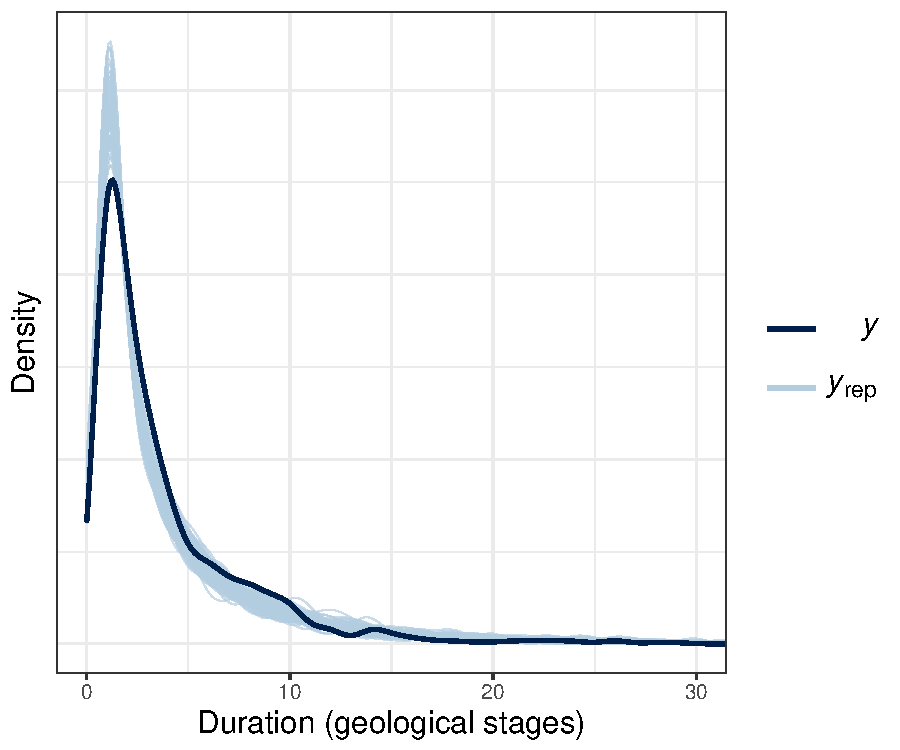
\includegraphics[height = 0.5\textheight,width=\textwidth,keepaspectratio=true]{figure/ppc_dens_zoom_cweib_cens}
  \caption{ Comparison of the distribution of the observed data (black) to 100 simulated distributions (blue). This is a close-up view of the bulk of the distribution which shows the more subtle aspects of (mis)fit between the data and the model. }
  \label{fig:dens_overlay_zoom}
\end{figure}


Comparisons between the survival functions estimated from the empirical data and from 100 simulated datasets further expands the picture of model (mis)fit (Fig. \ref{fig:surv}). The survival curves of the 100 simulated datasets are very similar to the survival function estimated from the empirical data. The major points of potential misfit between the model and the data are underestimated percentage of taxa with duration 1 stage, and an over-estimate of probability of species surviving at least 9-16 stages. Importantly, the major divergence between the observed and estimated applies to taxa with a less than 15\% probability of continuing to surviving. Keep in mind, also, that the survival curve as presented does not depict density of observations as in Fig. \ref{fig:dens_overlay_zoom}.

\begin{figure}[ht]
  \centering
  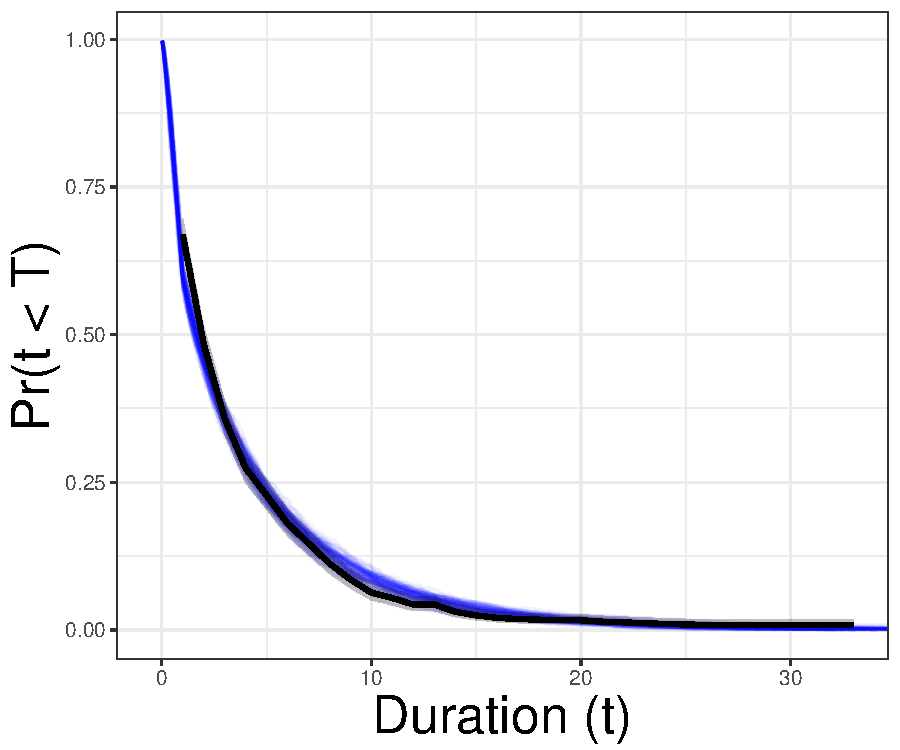
\includegraphics[height = 0.5\textheight,width=\textwidth,keepaspectratio=true]{figure/survival_curves_cweib_cens}
  \caption{Comparison of the empirical estimate of \(S(t)\) (highlighted) versus estimates from 100 posterior predictive data sets (black). \(S(t)\) corresponds to the probability that the age of a genus \(t\) is less than the genus' ultimate duration \(T\). }
  \label{fig:surv}
\end{figure}


In addition to distributional comparisons, model adequacy at the total data level was assessed through comparison of the mean and median of the observed data to those from simulated data sets. While the previous posterior predictive checks have focused on the relatively good but heterogeneous fit of the model to the entire distribution of the data, assessment of the models ability to predict the mean and median of the observed data appears adequate (Fig. \ref{fig:ppc_mean,fig:ppc_median}). The principle goal of this model is to obtain adequate prediction of how a taxon's expected duration for a given set of ecological covariates, as such the seemingly adequate fit of our model to average taxon duration is reassuring (Fig. \ref{fig:ppc_mean}). Additionally, given the skewness of the observed taxon durations (Fig. \ref{fig:dens_overlay_zoom}, the ability for the model to recapitulate the median observed taxon duration is important.

\begin{figure}[ht]
  \centering
  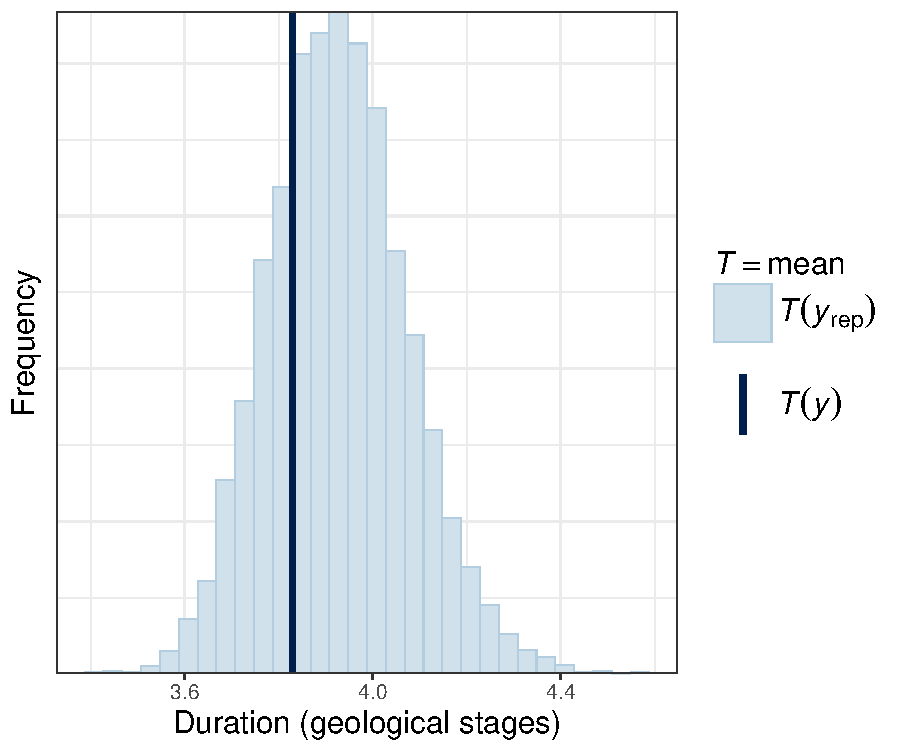
\includegraphics[height = 0.5\textheight,width=\textwidth,keepaspectratio=true]{figure/ppc_mean_cweib_cens}
  \caption{ Comparison of the observed mean genus duration (black vertical line) to a distribution of means estimated from 100 simulated datasets (blue). Model fit is evaluated by the similarity between the observed and the estimated, where good fit is demonstrated by the vertical line being ``within'' the simulated distribution. }
  \label{fig:ppc_mean}
\end{figure}

\begin{figure}[ht]
  \centering
  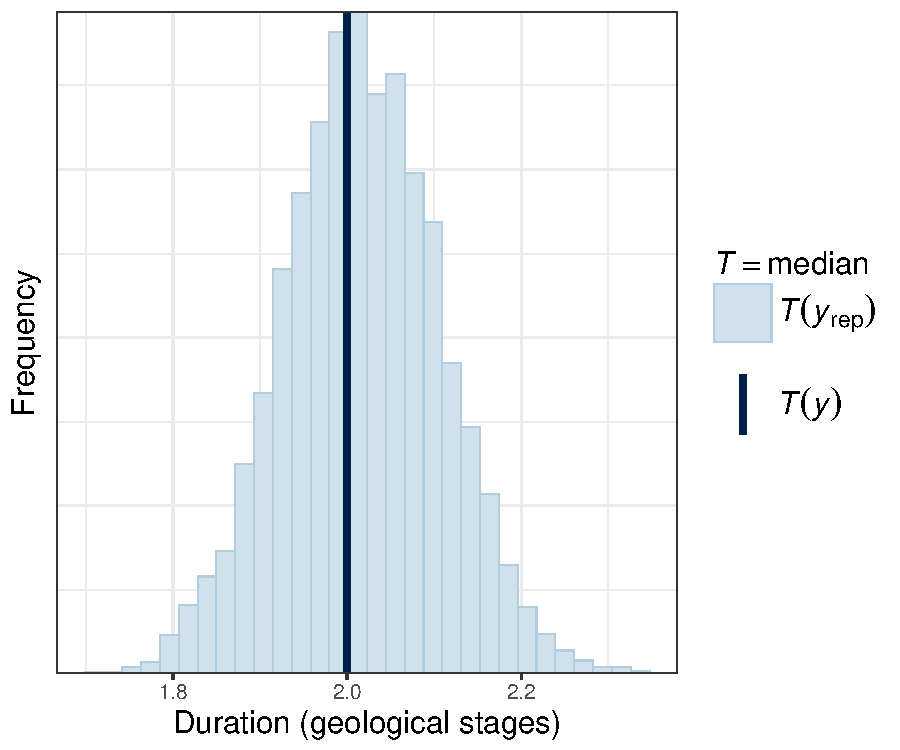
\includegraphics[height = 0.5\textheight,width=\textwidth,keepaspectratio=true]{figure/ppc_median_cweib_cens}
  \caption{ Comparison of the observed median genus duration (black vertical line) to a distribution of medians estimated from 100 simulated datasets (blue). Model fit is evaluated by the similarity between the observed and the estimated, where good fit is demonstrated by the vertical line being ``within'' the simulated distribution. }
  \label{fig:ppc_median}
\end{figure}


When considered together, all of the above posterior predictive checks indicate weak, but approximately adequate model fit for key questions such as expected taxon duration (Fig. \ref{fig:ppc_mean}). However, there is obviously heterogeneity in model fit because, while the model can recapitulate some aspects of the observed data (Fig. \ref{fig:ppc_mean,fig:ppc_median}), there are obvious discrepancies between the model and the data (Fig. \ref{fig:dens_overlay_zoom,fig:surv}). By performing the same posterior predictive tests for each of the origination cohorts, it may be possible to get a better picture of the source of model misfit.

When the posterior predictive tests are visualized for each of the origination cohorts, a complex picture of model fit emerges. Comparison between the empirical survival functions estimated for each cohort to those estimated from the simulated datasets reveals the degree of heterogeneity in model fit (Fig. \ref{fig:surv_group}, as some origination cohorts appear to be very well fit by the model (e.g. Tremadoc, Darriwilian Wenlock, Ludlow, Lochkovian, etc.) while others are more poorly fit by the model (e.g. Visean, Bashirian, Moscovian, Stephanian, Roadian, etc.). The poverty of model fit to these cohorts may indicate that these origination cohorts are undergoing a different extinction process whose aspects are unmodeled in this analysis. However, for those cohorts where our model recapitulates the empirical survival function indicates approximately adequate fit and that our model may be capturing some of the processes underlying taxon extinction.

% by origination cohort
\begin{figure}[ht]
  \centering
  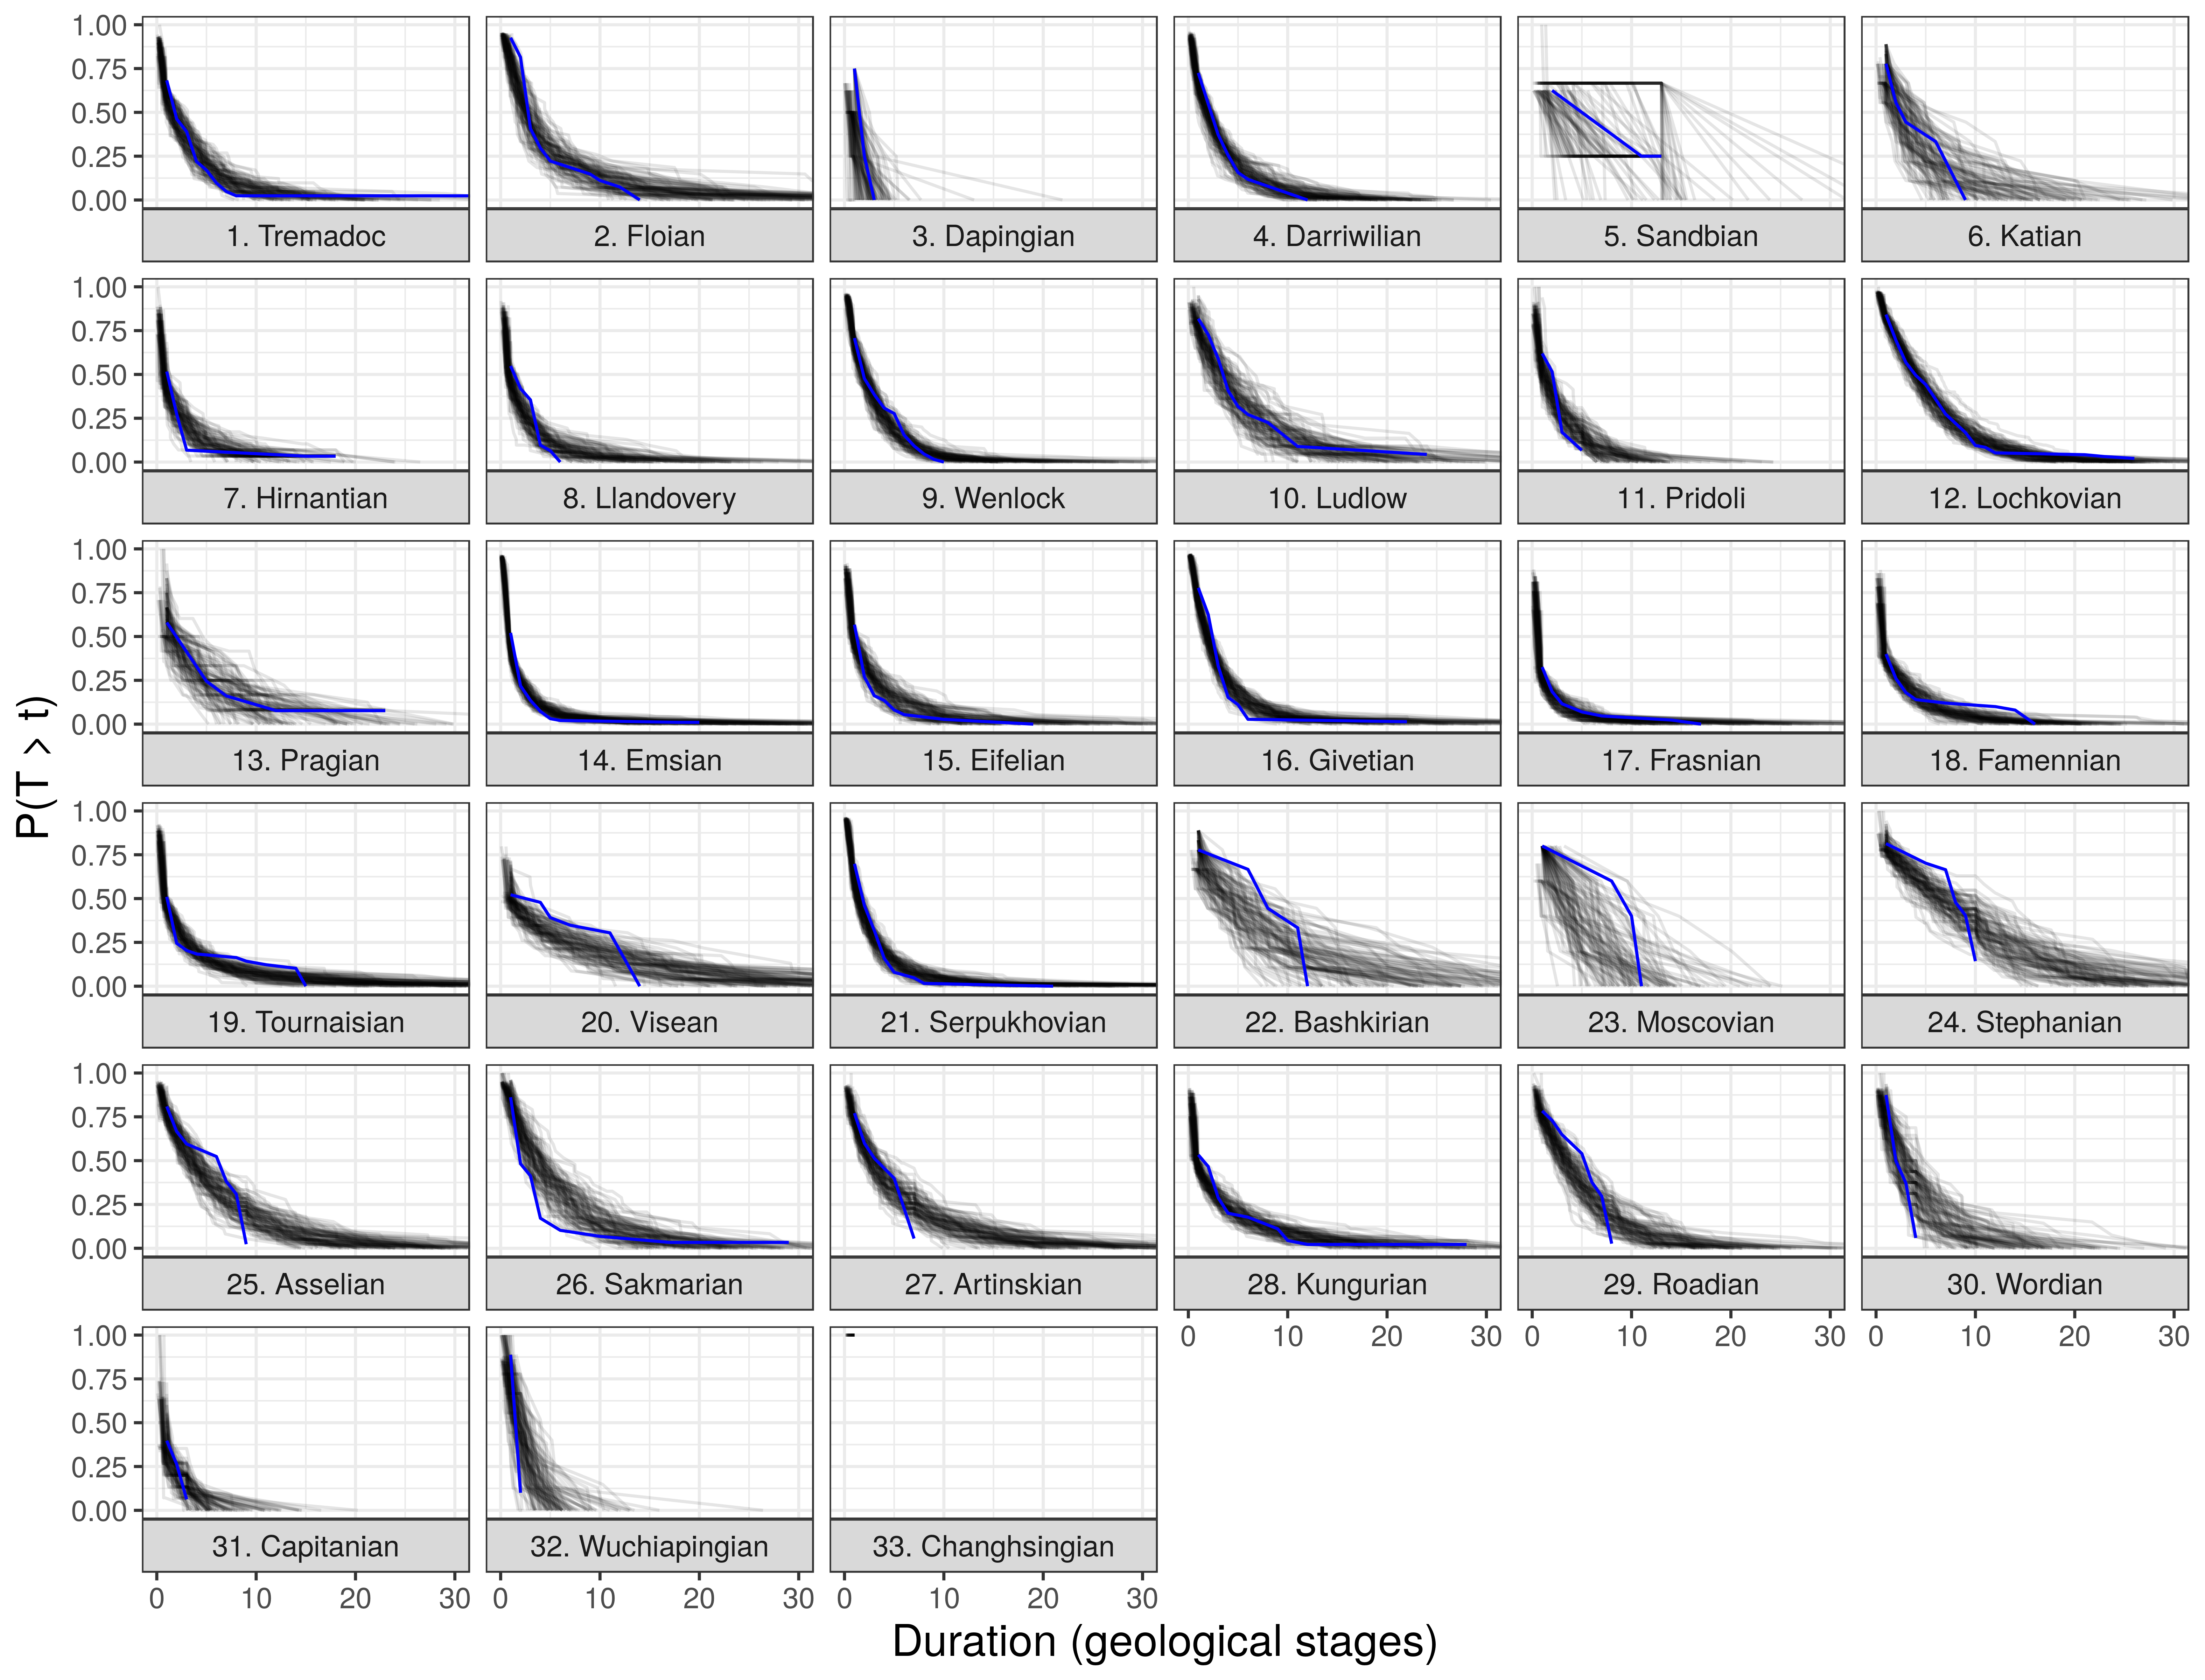
\includegraphics[height = 0.5\textheight,width=\textwidth,keepaspectratio=true]{figure/ppc_surv_coh}
  \caption{Comparison of the empirical estimate of \(S(t)\) (highlighted) versus estimates from 100 posterior predictive data sets (black) for each of the origination cohorts. \(S(t)\) corresponds to the probability that the age of a genus \(t\) is less than the genus' ultimate duration \(T\). By comparing the fit of the model to the individual cohorts, when and where the model (mis)fits is more observable. }
  \label{fig:surv_group}
\end{figure}


For nearly every origination cohort, the model is able to approximately recapitulate the observed mean duration (Fig. \ref{fig:group_mean}). The only exceptions to this observed mean is within the tails of the posterior predictive distributions (e.g. Moscovian, Sakmarian, Wordian, etc.). In general, however, posterior predictive distribution of the model is able to adequately estimate the mean duration of nearly all origination cohorts.

In comparison, the model has a much more heterogeneous fit to each origination cohort's median taxon duration (Fig. \ref{fig:group_median}). The skewness of the distribution underlying (Fig. \ref{fig:dens_overlay_zoom}) means that for some origination cohorts, median duration might be pegged at 1 stage; this means that the posterior predictive distributions for some cohorts can be extremely skewed. The cohorts with notably inadequate poor predictions are the Hirnantian, Priodoli, Emsian, Eifelian, Givetian, Asselian, Sakmarian, Artinskian, Kungarian, and Roadian. The remaining 13 cohorts, however, have decently adequate fit. These results indicate that our model is very good at recapitulate mean taxon duration (Fig. \ref{fig:ppc_mean}, \ref{fig:group_mean}), and it is capable of esimtaing overall median duration and median duration of most origination cohorts (Fig. \ref{fig:ppc_median}, \ref{fig:group_median}).

\begin{figure}[ht]
  \centering
  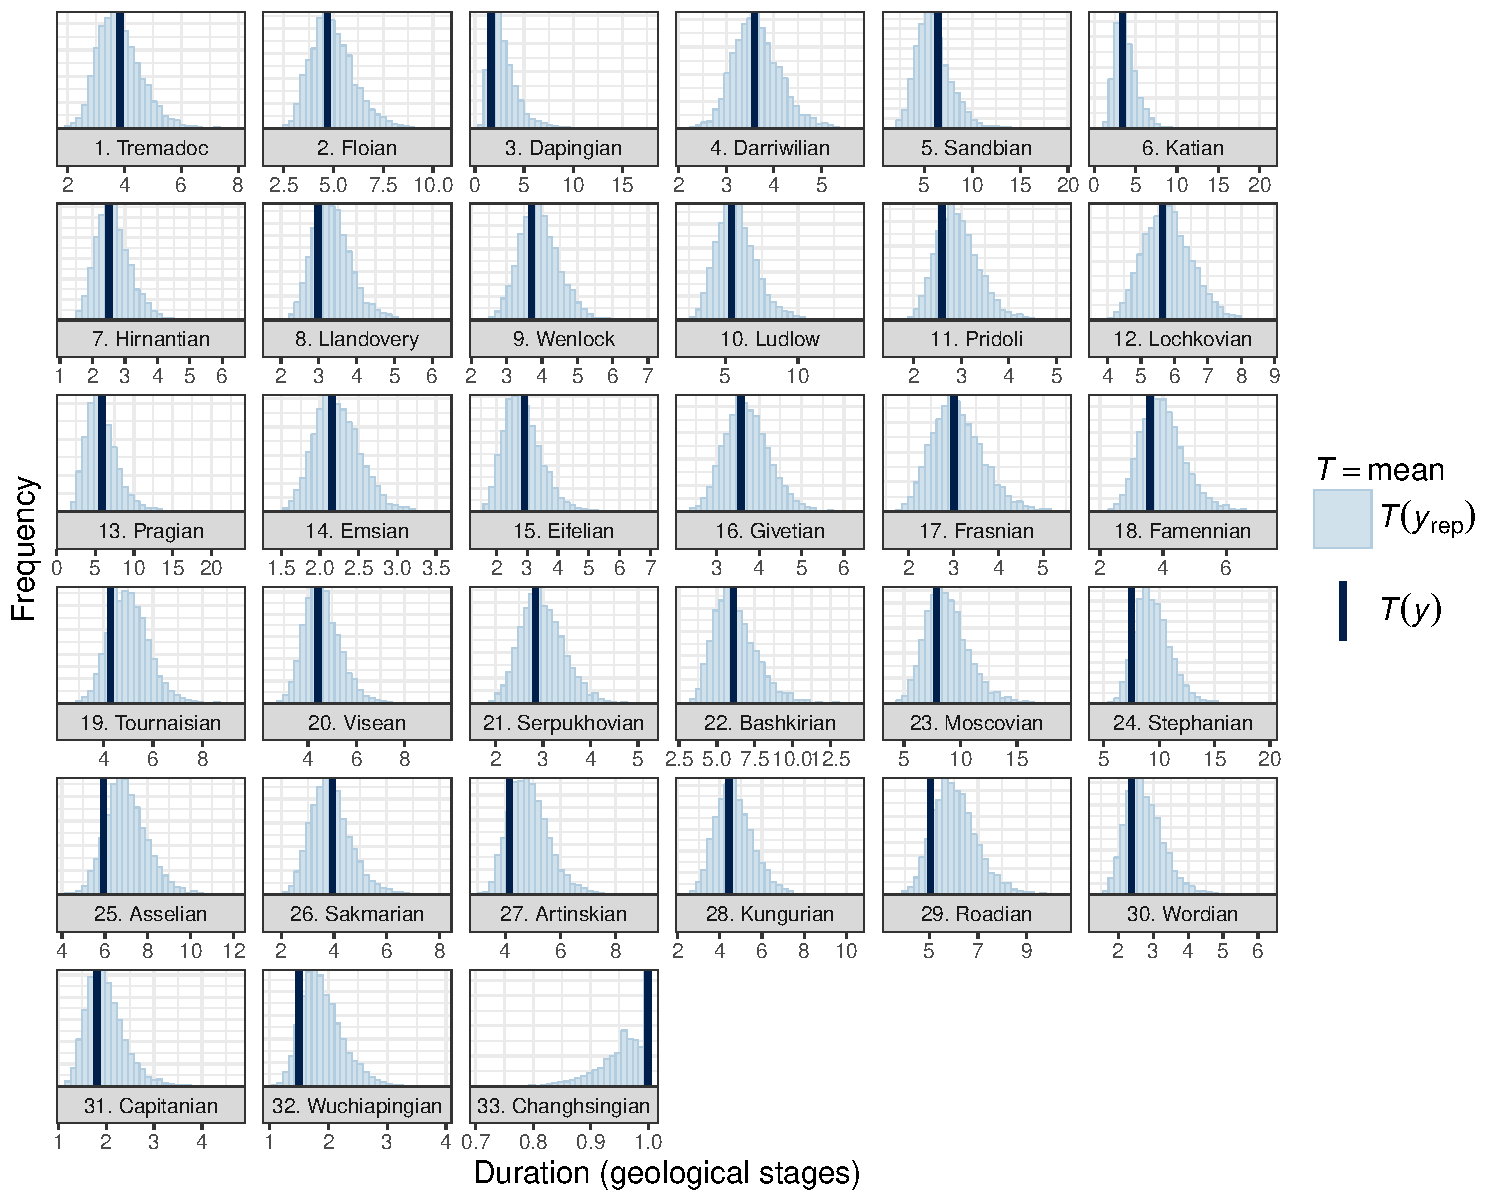
\includegraphics[height = 0.5\textheight,width=\textwidth,keepaspectratio=true]{figure/ppc_mean_group_cweib_cens}
  \caption{ Comparison of the observed mean genus duration (black vertical line) to a distribution of means estimated from 100 simulated datasets (blue) for each of the origination cohorts. Model fit is evaluated by the similarity between the observed and the estimated, where good fit is demonstrated by the vertical line being ``within'' the simulated distribution. }
  \label{fig:group_mean}
\end{figure}

\begin{figure}[ht]
  \centering
  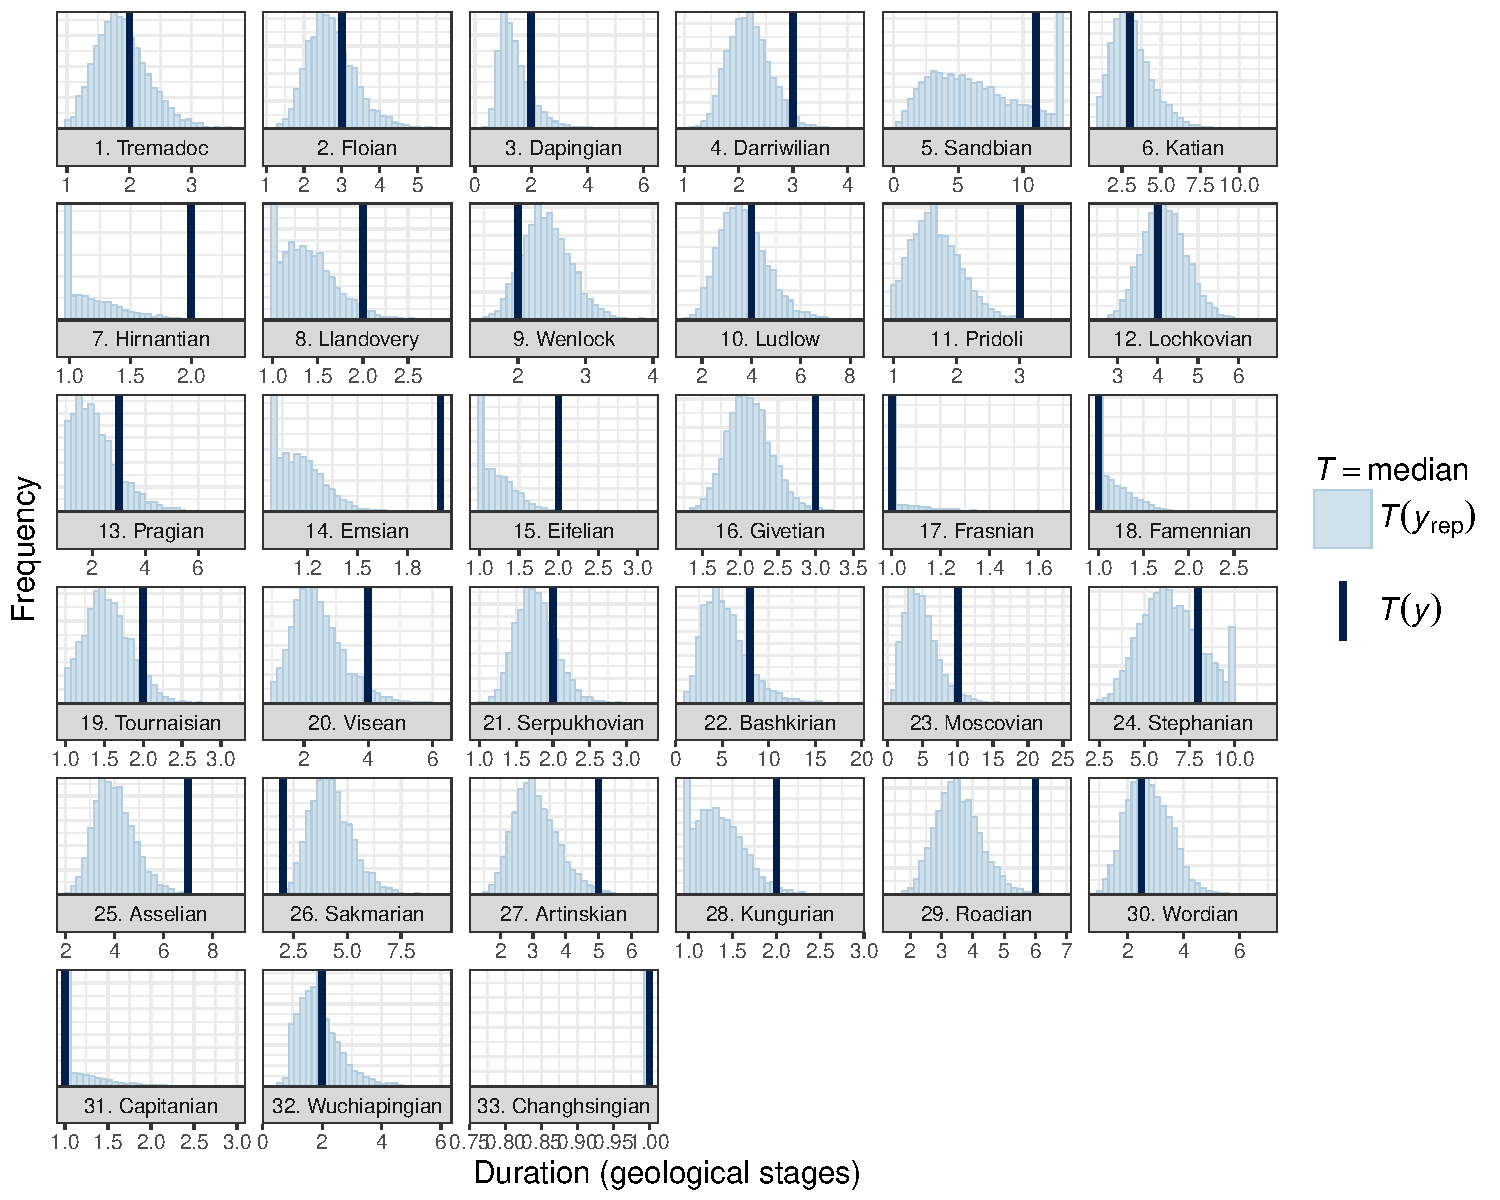
\includegraphics[height = 0.5\textheight,width=\textwidth,keepaspectratio=true]{figure/ppc_med_group_cweib_cens}
  \caption{ Comparison of the observed median genus duration (black vertical line) to a distribution of medians estimated from 100 simulated datasets (blue) for each of the origination cohorts. Model fit is evaluated by the similarity between the observed and the estimated, where good fit is demonstrated by the vertical line being ``within'' the simulated distribution. }
  \label{fig:group_median}
\end{figure}








%   testing biological hypotheses about extinction intensity and selectivity
%     ("if yes, if no" stuff could techically go in introducation as table. "these are important/relevant hypotheses that will be tested. here are the possible outcomes and possible explinations for those outcomes (with citations)")
%     geographic range
%       as range inc, duration inc? P(average effect > 0)
%         if yes:
%         if no:
%       could any cohort have reverse (range inc, duration desc)? P(any cohort effect < 0)
%         if yes:
%         if no:
%     environmental preference
%       two parts, hard to seperate; calculate on parabola
%       concave down?
%         if yes:
%         if no:
%       apex of curve favor epicontinental environments or open-ocean?
%         if yes:
%         if no:
%     correlation
%       as cohort's average duration inc, does cohort's average effect of geographic range inc? P(correlation > 0)
%         if yes:
%         if no:
%       as cohort's average duration inc, does cohort's average effect of favoring epi inc? P(correlation > 0)
%         if yes:
%         if no:
%       as cohort's average duration inc, does cohort's average curvature of the relationship inc? P(correlation > 0)
%         if yes:
%         if no:

\clearpage
\begin{table}[h]
%\begin{sidewaystable}
  \centering
  \caption{Estimates of various parameters in the model used here. These include group-level estimates of the effects of biological traits on brachiopod generic survival, the standard deviation of the between-cohort effects, as well as the estimates of both the effect of sampling \(\delta\) and the Weibull shape parameter \(\alpha\). The mean, standard deviation (SD), 10th, 50th, and 90th quantiles of the marginal posteriors are presented.}
  \begin{tabular}{ l | l p{2.5cm} r r r r r }
    \hline
    type & parameter & effect of & mean & SD & 10\% & 50\% & 90\% \\ 
    \hline
    \multirow{5}{*}{Mean} & \(\mu^{i}\) & intercept & -2.34 & 0.14 & -2.52 & -2.34 & -2.16 \\ 
    & \(\mu^{r}\) & geographic range &  1.19 & 0.21 & 0.93 & 1.19 & 1.45 \\ 
    & \(\mu^{v}\) & environmental preference &  -0.34 & 0.20 & -0.59 & -0.34 & -0.07 \\ 
    & \(\mu^{v^{2}}\) & environmental preference\(^{2}\) &  2.15 & 0.30 & 1.76 & 2.15 & 2.53 \\ 
    & \(\mu^{m}\) & body size & 0.05 & 0.11 & -0.09 & 0.05 & 0.19 \\ 
    \hline
    \multirow{5}{*}{Standard deviation} & \(\tau^{i}\) & intercept &  0.51 & 0.11 & 0.38 & 0.50 & 0.65 \\ 
    & \(\tau^{r}\) & geographic range & 0.77 & 0.17 & 0.55 & 0.75 & 1.00 \\ 
    & \(\tau^{v}\) & environmental preference & 0.97 & 0.18 & 0.76 & 0.95 & 1.20 \\ 
    & \(\tau^{v^{2}}\) & environmental preference\(^{2}\) &  1.08 & 0.34 & 0.66 & 1.07 & 1.52 \\ 
    & \(\tau^{m}\) & body size &  0.41 & 0.11 & 0.27 & 0.41 & 0.56 \\ 
    \hline
    \multirow{2}{*}{Other} & \(\delta\) & sampling & -2.77 & 0.15 & -2.97 & -2.77 & -2.58 \\ 
    & \(\alpha\) & ``time'' & 1.61 & 0.05 & 1.54 & 1.61 & 1.67 \\ 
    \hline
  \end{tabular}
  \label{tab:param}
\end{table}
%\end{sidewaystable}
\clearpage



The cohort-level estimate of the effect of geographic range size indicates that as a taxon's geographic range increases, that taxon's duration is expected to increase (Table \ref{tab:param}). Given the estimates of \(\mu^{r}\) and \(\tau^{r}\), there is an approximately 7\% (\(\pm 5\%\) SD) probability that this relationships would be reversed (\(\mathrm{Pr}\mathcal{N}(\mu^{r}, \tau^{r}) > 0)\)). 

Body size is estimated to have a slightly positive estimate, which means that species with greater than average size are expected to have a shorter duration than species with below average size (Table \ref{tab:param}).

The group-level estimate of the effect of environmental preference is estimated from both \(\mu^{v}\) and \(\mu^{v^{2}}\). The estimate of \(\mu^{v}\) indicates that epicontinental favoring taxa are expected to have a greater duration than open-ocean favoring taxa (Table \ref{tab:param}). Additionally, given the estimate of between-cohort variance \(\tau^{v}\), there is approximately 36.1\% (\(\pm 8\%\) SD) probability that, for any given cohort, taxa favoring open-ocean environments would have a greater expected duration than taxa favoring epicontinental environments (\(\mathrm{Pr}(\mathcal{N}(\mu^{v}, \tau^{v}) > 0)\)). The estimate of \(\mu^{v^{2}}\) indicates that the overall relationship between environmental preference and \(\log(\sigma)\) is concave down (Fig. \ref{fig:env_mean}), with only a 3.6\% (\(\pm 4\%\) SD) probability that any given cohort is convex up (\(\mathrm{Pr}(\mathcal{N}(\mu^{v^{2}}, \tau^{v^{2}}) < 0\)).

  \begin{figure}[ht]
  \centering
  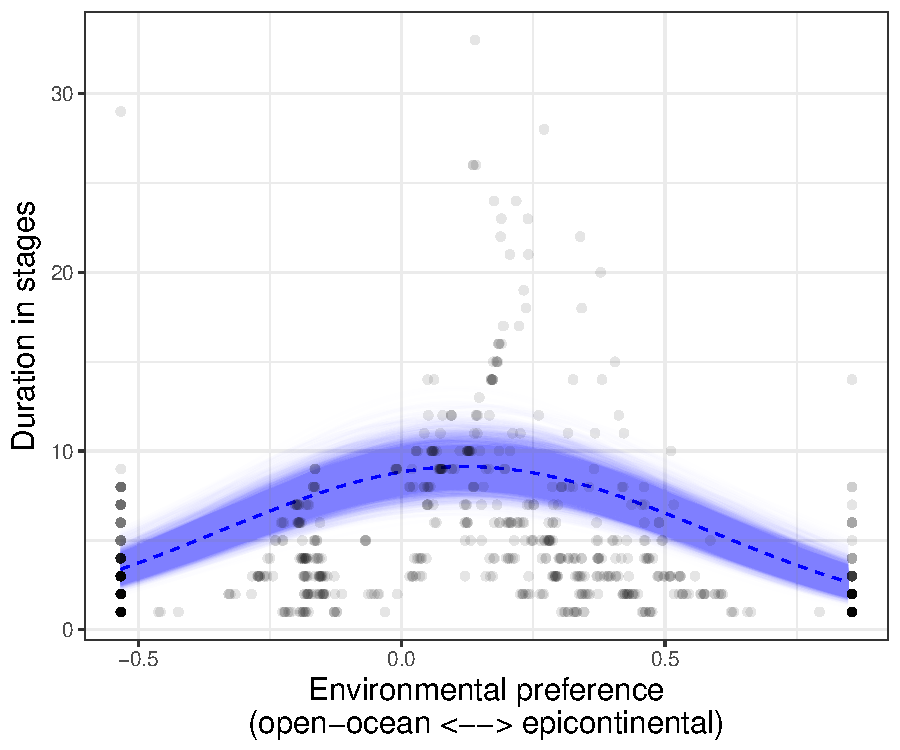
\includegraphics[height = 0.5\textheight,width=\textwidth,keepaspectratio=true]{figure/env_effect_med_cweib_cens}
  \caption{The overall expected relationship between environmental affinity \(v_{i}\) and a \(\log(\sigma)\) when r = 0 and m = 0. The 1000 semi-transparent lines corresponds to a single draw from the posterior predictive distribution, while the highlighted line corresponds to the median of the posterior predictive distribution. The overall relationship is concave down with an optimum greater than 0, which means that taxa favoring epicontinental environments are expected to have longer durations than those favoring open-ocean environments. The tick marks along the bottom of the plot correspond to the (rescaled) observed values of environmental preference.}
  \label{fig:env_mean}
\end{figure}



The cohort-specific estimates of all the regression coefficients demonstrate a lot of between cohort variance, with no obvious trends. %As indicated in Table \ref{tab:param} and detectable visually (Fig. \ref{fig:cohort_series}), the between-cohort estimates for \(\beta^{0}\), \(\beta^{r}\), and \(\beta^{m}\) all have much lower variance than the between-cohort estimates of both \(\beta^{v}\) and \(\beta^{v^{2}}\).


While most cohort-specific estimates are very similar to the overall cohort-level estimate, there are a few notable chorts for which two or more individual-level parameter estimates diverge greatly from the group-level averages (Fig. \ref{fig:cohort_series}). 


Wenlock \(\beta^{v}\) + and \(\beta^{m}\) -

There are simultaneous excursions in both \(\beta^{0}\) and \(\beta^{r}\) during the Pragian with \(\beta^{0}\) decreases while \(\beta^{r}\) increases. 

During the Emsian, there are excursions in \(\beta^{0}\), \(\beta^{r}\), and \(\beta^{m}\). 

Frasnian \(\beta^{v}\) - and \(\beta^{v^{2}}\) +

Famennian \(\beta^{0}\) -, \(\beta^{v}\) -

The Sakmarian is different from both the Pragian and Emsian in that \(\beta^{0}\), \(\beta^{r}\), \(\beta^{v}\), and \(\beta^{m}\) all have excursions from the group-average estimates.

Kungarian \(\beta^{v}\) - and \(\beta^{v^{2}}\) +


\begin{figure}[ht]
  \centering
  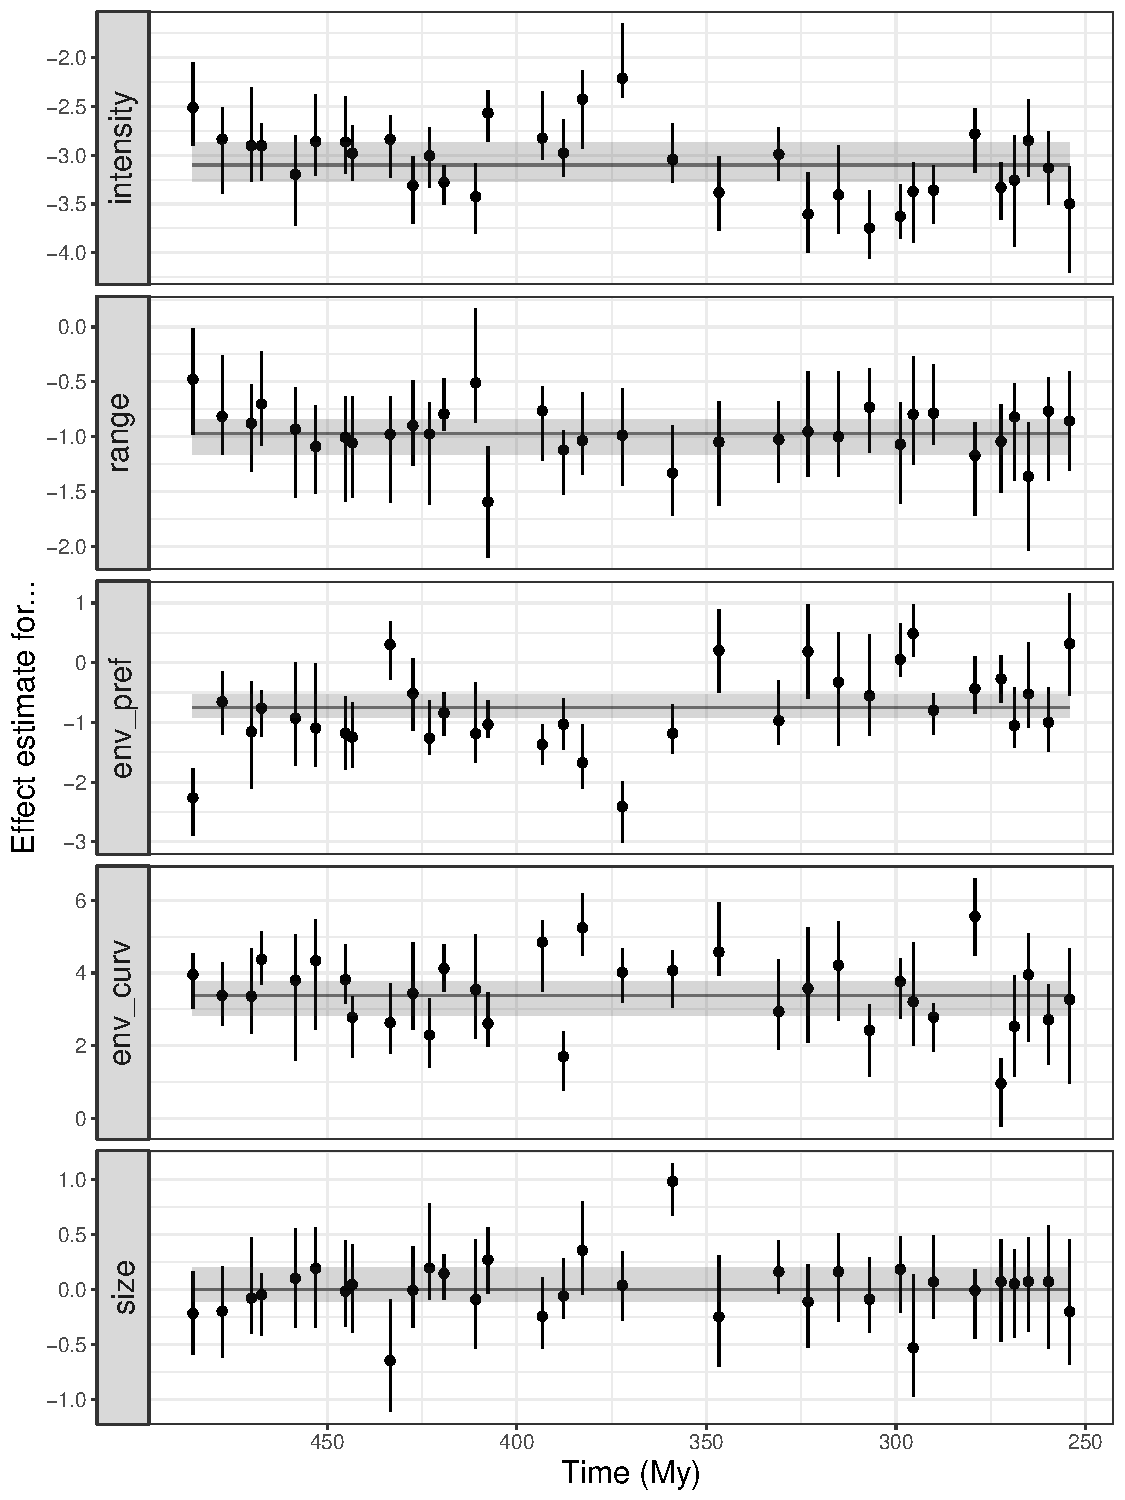
\includegraphics[width = \textwidth,height = 0.8\textheight,keepaspectratio=true]{figure/cohort_series_cweib_cens}
  \caption{Comparison of cohort-specific estimates of \(\beta^{0}\), the effect of geographic range on extinction risk \(\beta^{r}\), the effect of environmental preference \(\beta^{v}\) and \(\beta^{v^{2}}\), and body size \(\beta^{m}\). Points correspond to the median of the cohort-specific estimate, along with 80\% credible intervals. Points are plotted at the midpoint of the cohorts stage of origination in millions of years before present (My). Black, horizontal lines are the overall estimates of covariate effects along with 80\% credible intervals (shaded).}
  \label{fig:cohort_series}
\end{figure}



% cohort-specific environmental effect
%   description of the variation in estimates
%   mass extinction boundaries
The cohort-specific relationships between environmental preference and \(\log(\sigma)\) were calculated from the estimates of \(\beta^{0}\), \(\beta^{v}\), and \(\beta^{v^{2}}\) (Fig. \ref{fig:env_cohort}) and reflect how these three parameters act in concert and not just individually (Fig. \ref{fig:cohort_series}). 

%Beyond results already discussed above in the context of the parameters individually, it is notable that the cohort originating in the Kungurian (279-272 My) is least like the overall expected relationship and has the most sharply curved appearance due to a high estimate \(\beta^{v^{2}}\) (Fig. \ref{fig:cohort_series}). This cohort has the biggest difference in extinction risk between environmental generalists and specialists. The cohorts originating during the Emsian (407-393 My) and Frasnian (382 - 372 My) are tied for second in sharpness of curvature. The least sharply curved cohorts include those originating during Tremadocian (484-477 My), Hirnantian (445-443 My), Llandovery (443-433 My), and Ludlow (427-423 My). Except for the Tremadocian cohort, most of these cohorts originate during the Silurian through the Early Devonian range identified earlier as having lower expected extinction intensity than what is expected from the group-level estimate.

%The correlations of the cohort-specific estimates of the regression coefficients are estimated as the off-diagonal elements of the correlation matrix \(\Omega\). Only two of the elements of \(\Omega\) are distinguishable from 0: the correlation of \(\beta^{0}\) (extinction intensity) with both \(\beta^{r}\) and \(\beta^{v}\) (Fig. \ref{fig:cor_posterior}). 

%There is an approximate 90\% probability that the cohort-specific estimates of baseline extinction intensity \(\beta^{0}\) and the effect of geographic range \(\beta^{r}\) are negatively correlated; this means that for cohorts experiencing a lower extinction intensity (\(\beta^{0}\) decreases), the magnitude of the effect of geographic range is expected to decrease as well, and \textit{vice versa}; this is in contrast to the observation made by \citet{Jablonski1986} with regards to late Cretaceous bivalves.

\begin{figure}[ht]
  \centering
  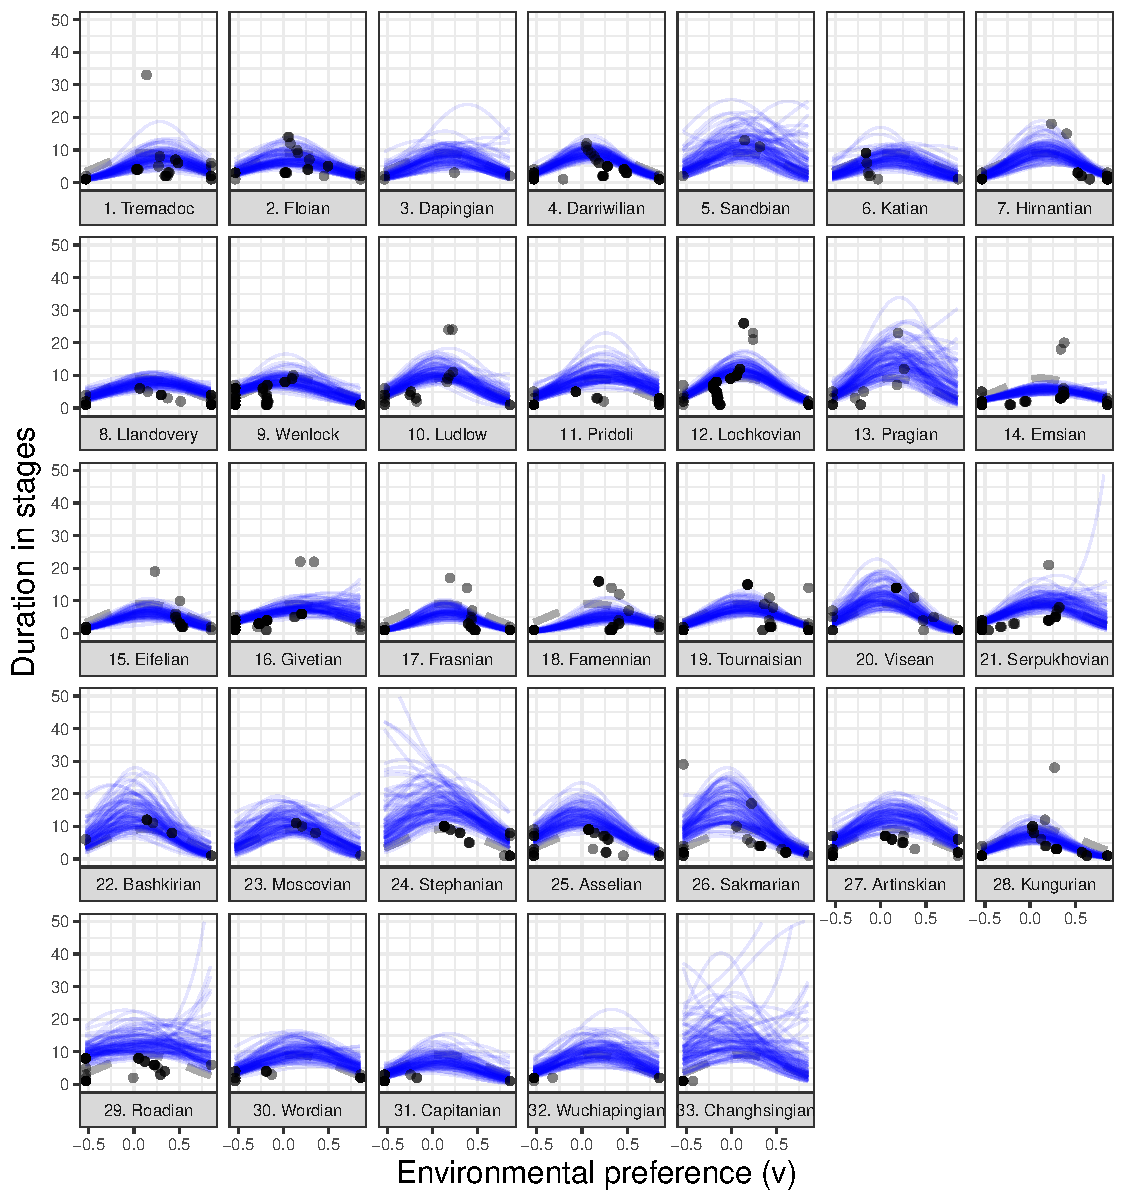
\includegraphics[width = \textwidth,height = 0.8\textheight,keepaspectratio=true]{figure/env_cohort_med_cweib_cens}
  \caption{Comparison of origination cohort-specific (posterior predictive) estimates of the effect of environmental preference on \(\log(\sigma)\) to the mean overall estimate of the effect of environmental preference. Cohort-specific estimates are from 100 posterior predictive simulations across the range of (transformed and rescaled) observed values of environmental preference. The oldest cohort is in the top-right and younger cohorts proceed left to right, with the youngest cohort being the right-most facet of the last row. Panel names correspond to the name of the stage in which that cohort originated.}
  \label{fig:env_cohort}
\end{figure}



Similarly, there is an approximate 99.5\% probability that the cohort-specific estimates of \(\beta^{0}\) and \(\beta^{v}\) are negatively correlated; this means that as extinction intensity increases it is expected that epicontinental taxa become more favored over open-ocean environments (i.e. as \(\beta^{0}\) increases, \(\beta^{v}\) decreases). 

There is only an approximate 60\% probability that \(\beta^{r}\) and \(\beta^{v}\) are positively correlated. This lack of cross-correlation may be due in part to the much higher between-cohort variance of the effect of environmental preference \(\tau^{v}\) than the very small between-cohort variance in the effect of geographic range \(\tau^{r}\) (Table \ref{tab:param}); the effect of geographic range might simply not vary enough relative to the much noisier environmental preference.

\begin{figure}[ht]
  \centering
  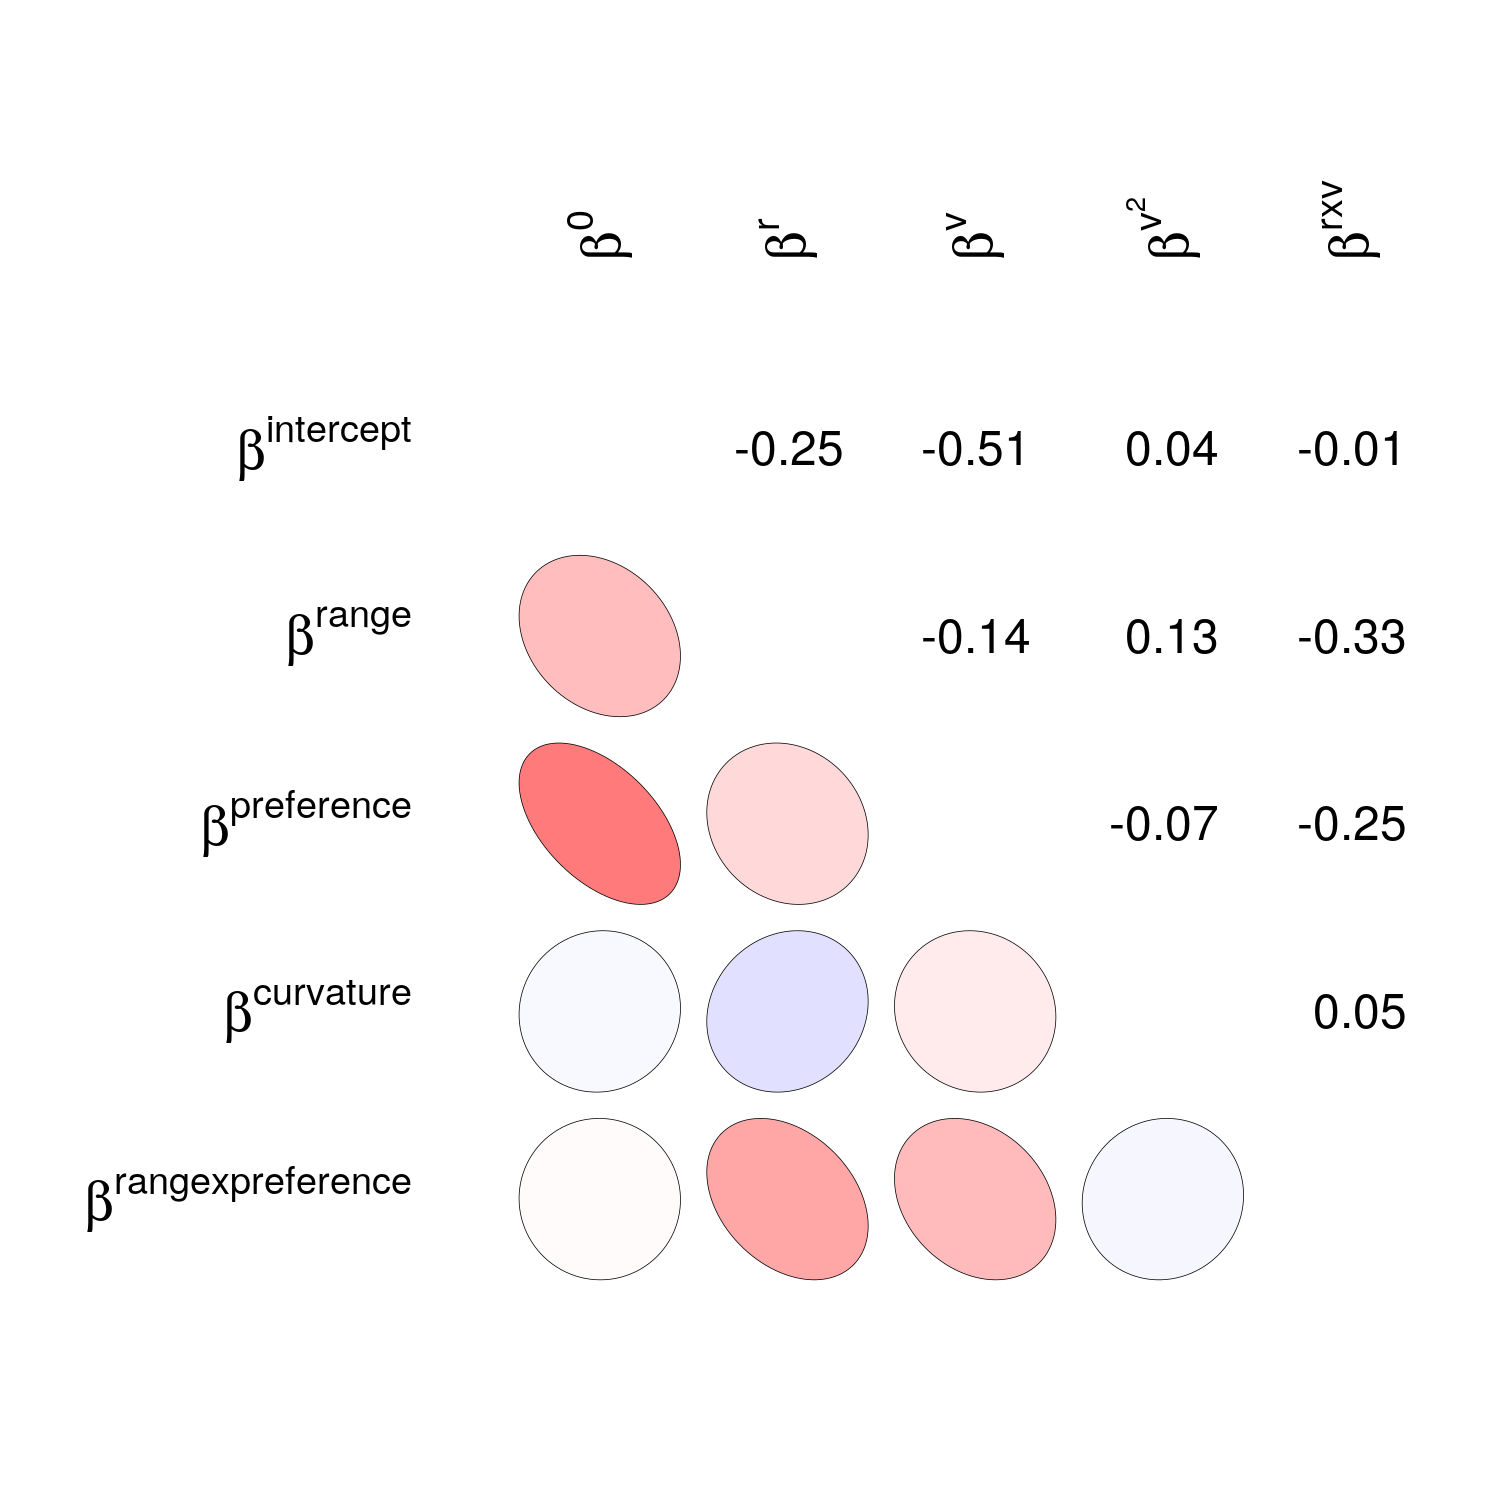
\includegraphics[height = 0.8\textheight,width=\textwidth,keepaspectratio=true]{figure/wei_cor_heatmap_cweib_cens}
  \caption{Mixed graphical and numerical representation of the correlation matrix \(\Omega\) of variation in cohort-specific covariate estimates. These correlations are between the estimates of the cohort-level effects of covariates, along with intercept/baseline extinction risk. The median estimates of the correlations are presented numerically (upper-triangle) and as idealized ellipses representing that much correlation (lower-triangle). The darkness of the ellipse corresponds to the magnitude of the correlation.}
  \label{fig:cor_posterior}
\end{figure}


Sampling was found to have a positive effect (negative \(\delta\)) on duration: greater sampling, shorter duration (Table \ref{tab:param}). While potentially counter intuitive, this result is most likely due to some long lived taxa only be sampled in the stages of the first and last appearance. Also, longer lived taxa have more opportunities to not be sampled than shorter lived taxa. These two factors will lead to this result. 


%While the effect of sampling appears large compared to the other regression coefficients, this is only because sampling was not standardized like the other covariates. To make the coefficients comparable, \(\delta\) is multiplied by twice the posterior mean of the standard deviation of sampling probability; the transformed value of \(\delta\) is then 0.642 (\(\pm 0.1\) SD). This effect is relatively small compared to the other covariate effects (Table \ref{tab:param}). There is then a 98.6\% probability that the effect of geographic range \(\mu^{r}\) has a greater magnitude than \(\delta\). Similarly, \(\mu^{v}\) has a 71.8\% probability of having a greater magnitude of effect than \(\delta\). Finally, \(\mu^{v^{2}}\) has a 100\% probability of having a greater magnitude of effect than \(\delta\).

The Weibull shape parameter \(\alpha\) was found to be approximately 1.61 (\(\pm 0.05\) SD) with a 100\% probability of being greater than 1. This result is not consistent with the Law of Constant Extinction \citep{VanValen1973} and is instead consistent with accelerating extinction risk with taxon age. This may indicate that older taxa are out-competed by younger taxa, a result consistent with some empirical results \citep{Wagner2014b,Quental2013,Smits2015} and (ironically) with a recently proposed Red Queen-like model of evolution \citep{Rosindell2015a}. This results, however, is not consistent with other empirical results \citep{Finnegan2008,Crampton2016} and could potentially be caused by the minimum resolution of the fossil record \citep{Sepkoski1975}. It is thus unclear if a strong biological inference can be made from this result, which means that further work is necessary on the effect of taxon age on extinction risk.




\section*{Discussion}

The generating observation behind this study was that for bivalves at the end Cretaceous mass extinction event, the only biological trait that was found the affect extinction risk was geographic range while traits that had previously been beneficial had no effect \citep{Jablonski1986}. This observation raises two linked questions: how does the effect of geographic range change with changing extinction intensity, and how does the effect of other biological traits change with changing extinction intensity?

I find that as intensity increases (\(\beta^{0}\) decreases), the magnitude of the effect of geographic range increases. I also find that as intensity increases, the effect of favoring epicontinental environments of open-ocean environments is expected to be increase; this is consistent with the results of \citet{Miller2009a}. There is no evidence for a correlation between the effect of geographic range and environmental preference. Additionally, the between-cohort variance in effect of geographic range is much less then the between-cohort variance of the effect of environmental preference which may underlie the lack of correlation between these two effects.

Additionally, the lower between-cohort variance in the effect of geographic range versus that higher between-cohort variance implies that for cohorts with a greater than average extinction intensity, the difference in the effect geographic range and the group-level effect of geographic range is expected to be smaller than the difference between the effect of environmental preference and the group-level effect of environmental preference.

I find consistent support for the ``survival of the unspecialized,'' with respect to epicontinental versus open-ocean environmental preference, as a time-invariant generalization of brachiopod survival; taxa with intermediate environmental preferences are expected to have lower extinction risk than taxa specializing in either epicontinental or open-ocean environments (Fig. \ref{fig:env_mean}), though the curvature of the relationship varies from rather shallow to very peaked (Fig. \ref{fig:env_cohort}). However, this relationship is not symmetric about 0, as taxa favoring epicontinental environments are expected to have a greater duration than taxa favoring open-ocean environments. This description of environment only describes one major aspect of a taxon's environmental context, with factors such as bathymetry and temperature being further descriptors of a taxon's adaptive zone \citep{Nurnberg2013a,Harnik2013,Harnik2011,Heim2011}; inclusion of these factors in future analyses would potentially improve our understanding of the ``survival of the unspecialized'' hypothesis \citep{Simpson1944}.

\citet{Hopkins2014a}, in their analysis of niche conservatism and substrate lithological preference in marine invertebrates, found that brachiopods were among the least ``conservative'' groups; taxa were found to easily change substrate preference on short time scales. While substrate preference is not the same as environmental preference (as defined here), a question does arise: are there three classes of environmental preference instead of two? These classes would be taxa with broad tolerance (``true'' generalists), inflexible specialists (``true'' specialists), and flexible but with a narrow tolerance. A flexible taxon is one with a narrow habitat preference at one time, but with preference that changes over time with changing environmental availability. My analysis assumes that traits are constant over the duration of the taxon meaning that this scenario is not detectable; taxa with broad tolerances and flexible taxa with narrow per-stage preference end up being treated the same way. Future work should explore how environmental preference changes over lineage duration in relation to environmental availability to estimate if the generalists--specialists continuum is actually ternary relationship.

An alternative approach for specifically modeling survival that can take into account imperfect observation than the method used here is the Cormack-Jolly-Seber (CJS) model \citep{Royle2008,Liow2008,Tomiya2013,Liow2010b}. This model is a type of hidden Markov model with an absorbing state (i.e. extinction). In this model, survival is defined as the probability of surviving from time \(t\) to time \(t + 1\). Additionally, the effect of preservation and sighting is estimated as probability of observing a taxon that is present; this can extend the duration of a taxon beyond its last occurrence. This approach is a fundamentally different from the method used in my analysis: I am estimating the biasing effect of sampling probability on taxon duration to then compare with effects of other covariates, while the CJS model estimates the pre-sampling fossil record and then estimates per-time unit survival probability.

% discussion of context of study
%   defense
%     species:genus?
%     difficulty towards tails, but that's to be expected
%       this model is about expectations, not tails/extreme events
%       this model is ok for the main part of the data
%       though, of course, this model has a long way to go (all models are false)
The use of genera as the unit of the study and how to exactly interpret the effects of the biological traits is an important question. For example, if any of the traits analyzed here are associated with increases in speciation rates, this might increase the duration of genera through self-renewal \citep{Raup1991b,Raup1994}, which would be an example of the difference in biological pattern between species and genera \citep{Jablonski1987,Jablonski2007,Jablonski2008a}. This could lead to a trait appearing to decrease generic level extinction risk by that trait increasing species level origination rate instead of decreasing species level extinction risk. % conflict between levels in effect: genus duration increased by speciation, not extinction of species

% future direction
The model used here could be improved through either increasing the number of analyzed traits, expanding the hierarchical structure of the model to include other major taxonomic groups of interest, and the inclusion of explicit phylogenetic relationships between the taxa in the model as an additional hierarchical effect. An example trait that may be of particular interest is the affixing strategy or method of interaction with the substrate of the taxon, which has been found to be related to brachiopod survival where, for cosmopolitan taxa, taxa that are attached to the substrate are expected to have a greater duration than those that are not \citep{Alexander1977}.

%   comparison with other major groups in hierarchical model
It is theoretically possible to expand this model to allow for comparisons both within and between major taxonomic groups which would better constrain the brachiopod estimates while also allowing for estimation of similarities and differences in cross-taxonomic patterns. The major issue surrounding this particular expansion involves finding a similarly well sampled taxonomic group that is present during the Paleozoic. Potential groups include Crinoidea, Ostracoda, and other members of the ``Paleozoic fauna'' \citep{Sepkoski1981a}.

With significant updates, it would also be possible to compare the brachiopod record with with Moden groups such as bivalves or gastropods \citep{Sepkoski1981a}, though remembering that the groups may not necessarily share all cohorts with the brachiopods. This particular model expansion would act as a test of any universal cross-taxonomic patterns in the effects of emergent traits on extinction such as has been proposed for geographic range \citep{Payne2007}. Additionally, this expanded model would also act as a test of the distinctness of the \citet{Sepkoski1981a} three-fauna hypothesis in terms of trait-dependent extinction.

Traits like environmental preference or geographic range \citep{Jablonski1987,Hunt2005b} are most likely heritable. Without phylogenetic context, this analysis assumes that differences in extinction risk between taxa are independent of the shared evolutionary history of those  taxa \citep{Felsenstein1985b}. In contrast, the origination cohorts only capture shared temporal context. For example, if taxon duration is phylogenetically heritable, then closely related taxa may have more similar durations as well as more similar biological traits. Without taking into account phylogenetic similarity the effects of these biological traits would be inflated solely due to inheritance. The inclusion of phylogenetic context as an additional individual-level hierarchical effect, independent of origination cohort, would allow for determining how much of the observed variability is due to shared evolutionary history versus shared temporal context versus actual differences associated with biological traits \citep{Smits2015}.

The combination and integration of the phylogenetic comparative and paleontological approaches requires both sources of data, something which is not possible for this analysis because there is no phylogenetic hypothesis for all Paleozoic taxa, something that is frequently the case for marine invertebrates with a good fossil record. When both data sources are available has been possible, however, the analysis can more fully address the questions of interest in macroevolution \citep{Smits2015,Slater2013a,Slater2015b,Simpson2011,Tomiya2013,Slater2012,Raia2013c,Raia2012f,Harnik2014,Fritz2013a}.

\section*{Conclusion}
% concluding statements
In summary, patterns of Paleozoic brachiopod survival were analyzed using a fully Bayesian hierarchical survival modelling approach while also eschewing the traditional separation between background and mass extinction. I find that cohort extinction intensity is negatively correlated with both the cohort-specific effects of geographic range and environmental preference. These results imply that as extinction intensity increases (\(\beta^{0}\)) increases, it is expected that both effects will increase in magnitude. However, the change in effect of environmental preference is expected to be greater than the change in the effect of geographic range. Additionally, I find support for greater survival in environmental generalists over specialists in all origination cohorts analyzed; this is consistent with the long standing ``survival of the unspecialized'' hypothesis \citep{Liow2004a,Liow2007b,Simpson1944,Simpson1953,Smits2015,Nurnberg2015,Nurnberg2013a, Baumiller1993}. The results of this analysis support the conclusion that for Paleozoic brachiopods, as extinction intensity increases overall extinction selectivity is expected to increase as well.






%%%%%%%%%%%%%%%%%%%%%
% Acknowledgments
%%%%%%%%%%%%%%%%%%%%%
% You may wish to remove the Acknowledgments section while your paper 
% is under review (unless you wish to waive your anonymity under
% double-blind review) if the Acknowledgments reveal your identity.
% If you remove this section, you will need to add it back in to your
% final files after acceptance.

\section*{Acknowledgments}

I would like to thank K. Angielzcyk, M. Foote, P. D. Polly, R. Ree, and G. Slater for helpful discussion during the conception of this study. I'd also like to thank D. Bapst, N. Pierrehumbert and M. Villarosa Garcia for additional comments. An additional thank you to  A. Miller for the epicontinental versus open-ocean assignments. Finally, thank you to the reviewers for their helpful comments that improved this manuscript. This entire study would would not have been possible without the Herculean effort of the many contributors to the Paleobiology Database. In particular, I would like to thank J. Alroy, M. Aberhan, D. Bottjer, M. Clapham, F. F\"{u}rsich, N. Heim, A. Hendy, S. Holland, L. Ivany, W. Kiessling, B. Kr\"{o}ger, A. McGowan, T. Olszewski, P. Novack-Gottshall, M. Patzkowsky, M. Uhen, L. Villier, and P. Wager. This work was supported by a NASA Exobiology grant (NNX10AQ446) to A. Miller and M. Foote. I declare no conflicts of interest. This is Paleobiology Database publication XXX. The code necessary for reproducing these results is avaliable as a Zenodo archive DOI 10.5281/zenodo.46928.

\newpage{}


\bibliographystyle{amnat}
\bibliography{newbib,packages}
%%%%%%%%%%%%%%%%%%%%%
% Bibliography
%%%%%%%%%%%%%%%%%%%%%
% You can either type your references following the examples below, or
% compile your BiBTeX database and paste the contents of your .bbl file
% here. The amnatnat.bst style file should work for this---but please
% let us know if you run into any hitches with it!
% The list below includes sample journal articles, book chapters, and
% Dryad references.

%\begin{thebibliography}{}
%
%\bibitem[{Cook et~al.(2015)Cook, Collaborator, and Expert}]{CookEtAl2015}
%Cook, O.~E., G.~H. Collaborator, and A.~Q. Expert. 2015.
%\newblock Data from: Template and guidelines for using \LaTeX{} in \textit{The American Naturalist}.
%\newblock American Naturalist, Dryad Digital Repository, http://dx.doi.org/10.5061/dryad.XYZAB.
%
%\bibitem[{Davis et~al.(2011)Davis, Brakora, and Lee}]{DavisEtAl2011}
%Davis, E.~B., K.~A. Brakora, and A.~H. Lee. 2011.
%\newblock Evolution of ruminant headgear: a review.
%\newblock Proceedings of the Royal Society B 278:2857--2865.
%
%\bibitem[{Inglis et~al.(2011)Inglis, Roberts, Gardner, and Buckling}]{Ing11}
%Inglis, R.~F., P.~G. Roberts, A.~Gardner, and A.~Buckling. 2011.
%\newblock Spite and the scale of competition in \textit{Pseudomonas
%  aeruginosa}.
%\newblock American Naturalist 178:276--285.
%
%\bibitem[{Lemod\`{e}le et~al.(2007)Lemodele, Kapitelschreiber, and Exemplar}]{LemKapEx07}
%Lemod\`{e}le, P.-Q., A.~B. Kapitelschreiber, and C.~D.~E. Exemplar. 2007.
%\newblock An exemplary instance of chapters in books.
%\newblock Pages 231--245 \emph{in} J.-P. \'{E}crivain and M.~A. Term\'{e}szettud\'{o}s, eds. Inspiring Instances of Brilliant Writing. Truth Pudding Press, Fond du Lac, WI.
%
%\bibitem[{Xiao et~al.(2015)Xiao, McGlinn, and White}]{Xiao2015}
%Xiao, X., D.~J. McGlinn, and E.~P. White. 2015.
%\newblock A strong test of the maximum entropy theory of ecology.
%\newblock American Naturalist 185:E705--E80.
%
%\end{thebibliography}
%
%\newpage{}
%
%\section*{Tables}
%\renewcommand{\thetable}{\arabic{table}}
%\setcounter{table}{0}
%
%\begin{table}[h]
%\caption{Animals in various cities with equations}
%\label{Table:Okapi}
%\centering
%\begin{tabular}{llc}\hline
%Animal    & City         & Equation \\ \hline
%Dog       & Springfield  & $x+y=z$ \\
%Fox       & Indianapolis & $2x+2y=2z$ \\
%Okapi$^a$ & Chicago      & $x-y<z$ \\
%Badger    & Madison      & $x+2y>z$ \\ \hline
%\end{tabular}
%\bigskip{}
%\\
%{\footnotesize Note: Table titles should be short. Further details should go in a `notes' area after the tabular environment, like this. $^a$ Okapis are not native to Chicago, but they are to be met with in both of the major Chicagoland zoos.}
%\end{table}
%
%\newpage{}
%
%\section*{Figure legends}
%
%\begin{figure}[h!]
%%\includegraphics{horn-of-okapi}
%\caption{Figure legends can be longer than the titles of tables. However, they should not be excessively long.}
%\label{Fig:OkapiHorn}
%\end{figure}
%
%
%\begin{figure}[h!]
%%\includegraphics{elegance}
%\caption{In this way, figure legends can be listed at the end of the document, with references that work, even though the graphic itself should be included for final files after acceptance. Instead, upload the relevant figure files separately to Editorial Manager; Editorial Manager should insert them at the end of the PDF automatically.}
%\label{Fig:AnotherFigure}
%\end{figure}
%
%\subsection*{Online figure legends}
%
%\renewcommand{\thefigure}{A\arabic{figure}}
%\setcounter{figure}{0}
%
%\begin{figure}[h!]
%%\includegraphics{jumps20m}
%\caption{\textit{A}, the quick red fox proceeding to jump 20~m straight into the air over not one, but several lazy dogs. \textit{B}, the quick red fox landing gracefully despite the skepticism of naysayers.}
%\label{Fig:Jumps}
%\end{figure}
%
%\begin{figure}[h!]
%%\includegraphics{jumps20m}
%\caption{The quicker the red fox jumps, the likelier it is to land near an okapi. For further details, see \citet{LemKapEx07}.}
%\label{Fig:JumpsOk}
%\end{figure}
%
%\renewcommand{\thefigure}{B\arabic{figure}}
%\setcounter{figure}{0}
%
%\end{document}

\clearpage







\end{document}
